% Canonical HVK main manuscript. Detailed ablations and extended validation
% belong in supplementary_study.tex and should not be duplicated here.
\documentclass[journal]{IEEEtran}
\usepackage{amsmath,amsfonts,amssymb,graphicx,booktabs,cite,bm}
\usepackage[hidelinks,hypertexnames=false]{hyperref}
\usepackage{float}
\usepackage{flushend}
\hypersetup{
  pdftitle={Hamiltonian Vision Kernel: Symmetry, Entangling Correlators, and Real-Hardware Replay in Hybrid Quantum Image Reconstruction},
  pdfauthor={Sparsho Chakraborty and Siddhartha Patra},
  pdfsubject={Hybrid quantum-classical image reconstruction},
  pdfkeywords={quantum image processing, variational quantum circuits, tensor networks, equivariance, quantum hardware}
}
\begin{document}

\title{Hamiltonian Vision Kernel: Symmetry, Entangling Correlators, and Real-Hardware Replay in Hybrid Quantum Image Reconstruction}

\author{Sparsho~Chakraborty\IEEEauthorrefmark{1} and Siddhartha~Patra\IEEEauthorrefmark{2}%
\thanks{\IEEEauthorrefmark{1}School of Basic Sciences, Department of Physics, Indian Institute of Technology Bhubaneswar, Odisha, India.}%
\thanks{\IEEEauthorrefmark{2}Centre for Quantum Engineering, Research and Education (CQUERE), TCG CREST, Kolkata, India.}}

\maketitle

\begin{abstract}
We introduce the Hamiltonian Vision Kernel (HVK), a physics-informed framework for hybrid quantum--classical visual representation and reconstruction. HVK combines matrix-product-state patch features, a variational quantum circuit exposing a Pauli-correlator latent space, two-dimensional Fourier positional encoding, a learnable Hamiltonian energy diagnostic, and a classical decoder. HVK1D and HVK2D instantiate chain and grid interaction graphs, while observable pooling provides $D_4$ equivariance by construction. In a scoped three-image-per-dataset study across six real image datasets, the framework supports high-fidelity per-image reconstruction. Three results characterize its structure. First, the pooled HVK2D map achieves numerical equivariance error of $9.57\times10^{-17}$. Second, across five seeds on a leakage-audited task requiring distant-patch products, the entangling observable channel reaches mean $R^2=0.974$, compared with $R^2\leq0.02$ for non-entangling controls. Third, five images are reconstructed from observables measured on IBM Quantum hardware without retraining, reaching $25.90$--$31.52$~dB PSNR. Fourth, exploratory training-dynamics diagnostics --- a magnetization-style change-point statistic and an energy-to-entanglement ratio, tracked across training and varied along qubit-count ($N=4,6,8$) and, separately, MPS-bond-dimension ($\chi=1,2,4,8$) axes in noiseless simulation --- are additionally replayed across the qubit-count axis via gate-for-gate checkpoint reconstruction on real IBM Quantum hardware; these are descriptive, small-sample results, not inferential evidence of a thermodynamic phase transition. These results motivate HVK as a framework for studying symmetry, topology, nonlocal correlations, Hamiltonian diagnostics, and hardware-executed visual models. A companion supplementary study provides resource-matched held-out controls, leakage audits, statistical controls, and complete hardware methodology.
\end{abstract}

\begin{IEEEkeywords}
Quantum Image Processing, Tensor Networks, Variational Quantum Algorithms, Pauli Observables, Hamiltonian Diagnostics, Group-Equivariant Representations, Hybrid Quantum Hardware Validation.
\end{IEEEkeywords}

\section{Introduction}
Hybrid quantum--classical models for vision tasks are increasingly proposed as a route to representations with favorable inductive bias, exploiting entanglement, physically motivated regularizers, or tensor-network structure that classical convolutional pipelines do not natively expose \cite{Cerezo2021, Tilly2022, Preskill2018}. The variational quantum eigensolver and its descendants exploit the local decomposability of physically relevant Hamiltonians to construct shallow, problem-aware circuits \cite{Cerezo2021, Tilly2022, Bauer2020}, and quantum image processing provides encodings that place pixel information directly into qubit registers \cite{Chakraborty2018, Zhou2017, Yao2017}. Tensor-network methods, in parallel, have proven effective as compressed representations of structured classical data, including images \cite{Cirac2021, Latorre2005, Han2018, Stoudenmire2016, Fei2021, Guala2023}, and more broadly other structured data such as particle-physics events \cite{Araz2022}. Related hybrid quantum architectures target adjacent imaging tasks, including quantum annealing-based tomographic reconstruction \cite{Haga2024}, adiabatic quantum computing for emission tomography \cite{Nau2023}, quantum neural compressive sensing for ghost imaging \cite{Zhai2025}, hybrid autoencoder-plus-quantum-SVM feature extraction for image classification \cite{Slabbert2024}, and quantum capsule networks \cite{Liu2022}. HVK focuses on the specific combination of a Pauli-correlator latent space, enforced group-equivariant pooling, and a physically motivated energy diagnostic.

We introduce the Hamiltonian Vision Kernel (HVK1D/HVK2D), which combines these ingredients into a single architecture with three properties studied jointly here: a \emph{Pauli-correlator latent space} (measured VQC observables, not a raw quantum state, form the representation handed to a classical decoder, in the spirit of quantum-enhanced feature maps \cite{Havlicek2019}); an \emph{enforced, provable $D_4$ symmetry} extension, group-averaging the observable grid over the eight symmetries of the square rather than merely motivating symmetry through architecture choices, in the spirit of group-equivariant classical vision \cite{Cohen2016} and symmetry-embedding constructions for variational circuits \cite{Meyer2023}; and a \emph{learnable Hamiltonian energy diagnostic} (full nearest-neighbor $XX/YY/ZZ$ sectors in HVK1D and grid-edge $ZZ$ terms in HVK2D). Table~\ref{tab:differentiation} contrasts these properties against classical, adversarial, and standard quantum autoencoder baselines.

\paragraph{Contributions.}
\noindent\textbf{1) Architecture:} HVK1D/HVK2D combines MPS patch features, a six-qubit VQC, a 19--27-dimensional Pauli-correlator vector, 2D Fourier positional encoding, a graph-Hamiltonian diagnostic, and a classical decoder.

\noindent\textbf{2) Reconstruction scope:} Identically configured per-image fitting experiments cover six real image datasets (Section~\ref{sec:sameset_results}).

\noindent\textbf{3) Provable symmetry:} Group pooling makes the HVK2D observable map $D_4$-equivariant by construction and to floating-point precision numerically (Section~\ref{sec:d4}).

\noindent\textbf{4) Restricted nonlocal result:} In a leakage-audited fixed-readout protocol, entangling pair observables are necessary when the target depends explicitly on distant-patch products (Section~\ref{sec:entanglement_necessity}).

\noindent\textbf{5) Hardware pilot:} Five fitted checkpoints are replayed on IBM hardware without retraining and decoded from hardware-measured observables (Section~\ref{sec:hardware_pilot}).

\noindent\textbf{6) Training-dynamics diagnostics, in simulation and on real hardware:} A magnetization-style change-point statistic and an energy-to-entanglement ratio are tracked across training and varied along qubit-count ($N=4,6,8$) and, separately, MPS-bond-dimension ($\chi=1,2,4,8$) axes in simulation; the qubit-count axis is additionally replayed via gate-for-gate checkpoint reconstruction on real IBM Quantum hardware and the IonQ simulator across three shot budgets (Sections~\ref{sec:phase_transition}--\ref{sec:checkpoint_hardware_energy_entanglement}). These are descriptive, small-sample diagnostics --- not inferential evidence of a thermodynamic transition --- reported with the same detection formalism throughout (Eq.~\ref{eq:critical_epoch}).
A companion document, \textit{Supplementary Material for the Hamiltonian Vision Kernel: Resource-Matched Ablations, Validation, and Reproducibility}, reports resource-matched held-out comparisons of HVK and classical/ablated feature maps, together with full hardware-pilot methodology (circuit construction, validation, job identifiers, quota accounting) and explicit provenance audits of excluded exploratory results. We keep that analysis in a companion document so the architecture-level contributions above and the generalization question do not obscure each other; Section~\ref{sec:ablation_relationship} summarizes its central finding and how it relates to the results here.

\section{Hamiltonian Vision Kernel: Architecture}
\label{sec:architecture}
HVK treats each spatial patch as a finite spin state, compresses it as a matrix product state (MPS), measures a fixed set of Pauli observables from a variational quantum circuit (VQC), and decodes those observables back into pixels with a classical multi-layer perceptron (MLP). A learnable graph-Hamiltonian energy term regularizes training; unlike parameterized Hamiltonian learning approaches that treat the Hamiltonian as the primary learned object \cite{Shi2022}, HVK's energy term is a diagnostic regularizer alongside a separate reconstruction objective. The shared pipeline is:
\begin{equation}
\begin{aligned}
\text{Image} &\rightarrow \{\text{Patches}\} \rightarrow \text{MPS}\\
&\rightarrow \text{46-D/22-D Feature} \rightarrow \text{6-D Vector}\\
&\rightarrow \text{27-D/19-D Latent} \rightarrow \text{Decoder}\\
&\rightarrow \text{Reconstruction}.
\end{aligned}
\end{equation}
Two executed preprocessing configurations share this pipeline. For the $256\times256$ \textit{Monalisa}/HVK1D benchmark, sixteen non-overlapping $64\times64$ patches are $\ell_2$-normalized, reshaped as 12-site spin states, and sequentially SVD-compressed to MPS bond dimension $\chi=4$. Their 24 local $X/Z$ expectations, 11 nearest-neighbor $ZZ$ correlations, and 11 bipartite entropies form a 46-D feature vector. For the native $32\times32$ HVK2D multi-dataset experiments, sixteen $8\times8$ patches are represented by six-site MPSs, giving 12 local expectations, five nearest-neighbor $ZZ$ terms, and five entropies (22 dimensions). A learned linear layer compresses either MPS feature vector to six circuit angles. HVK1D then measures 27 observables (six local $Z$, six local $X$, and five each of $ZZ$, $XX$, and $YY$); HVK2D measures 19 (six local $Z$, six local $X$, and seven grid-edge $ZZ$ terms). The respective Fourier positional vectors have dimension eight and four. In both configurations, a two-hidden-layer MLP (128 and 256 units) maps the observable and positional vectors to one grayscale patch. Figure~\ref{fig:hvk_ansatz} shows the exact HVK1D and HVK2D ansatz circuits (rebuilt in Qiskit and numerically verified against the training-time PennyLane circuit as part of the hardware pilot of Section~\ref{sec:hardware_pilot}); complete Hamiltonian, loss, positional-encoding, and measurement definitions are retained in the companion supplement.

\begin{figure*}[t]
\centering
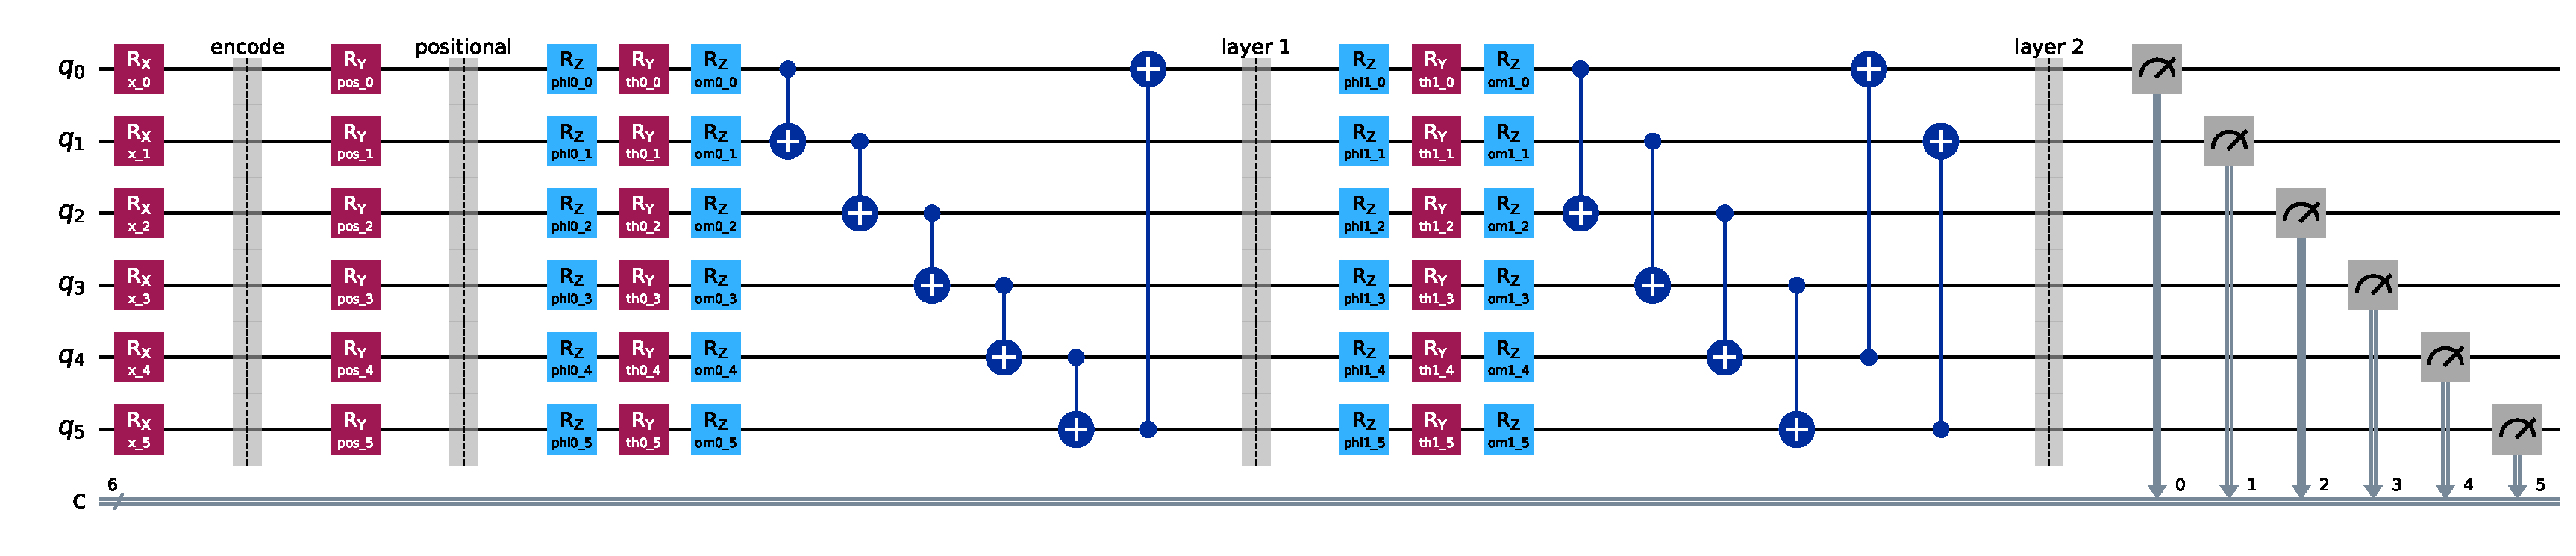
\includegraphics[width=0.95\textwidth]{figures/hvk1d_ansatz.pdf}\\[4pt]
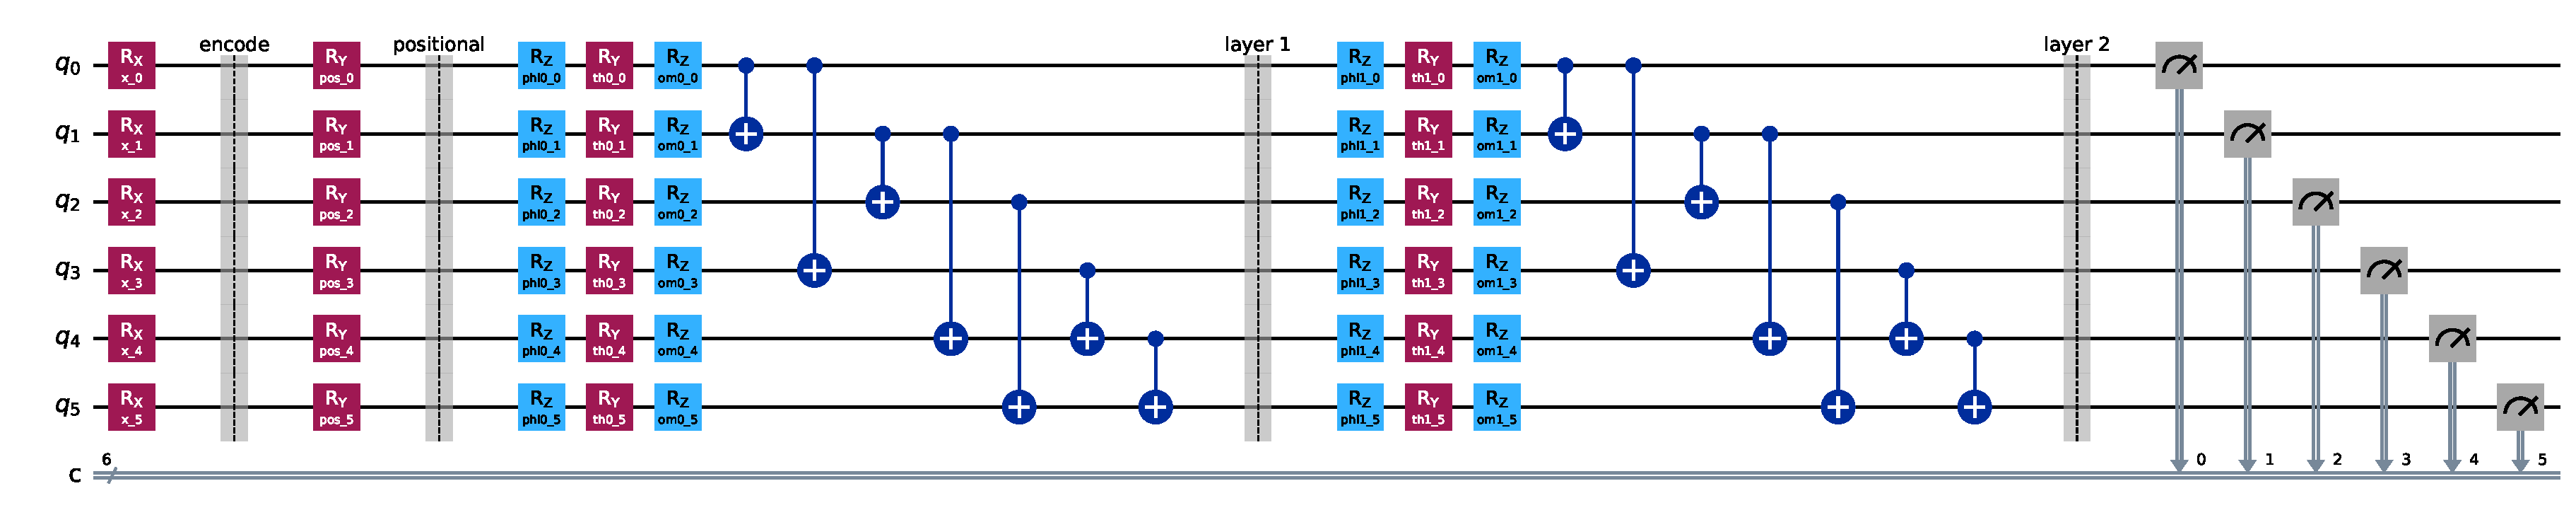
\includegraphics[width=0.95\textwidth]{figures/hvk2d_ansatz.pdf}
\caption{The HVK1D (top) and HVK2D (bottom) variational ansätze, exactly as executed (encoding $R_X$ rotations, positional $R_Y$ rotations, then two entangling layers of $R_Z$-$R_Y$-$R_Z$ single-qubit rotations with a CNOT ring for HVK1D or fixed grid-edge CNOTs for HVK2D). Both circuits were rebuilt gate-for-gate in Qiskit and validated against the original PennyLane training circuit before use in the hardware pilot of Section~\ref{sec:hardware_pilot}.}
\label{fig:hvk_ansatz}
\end{figure*}

Table~\ref{tab:variants} summarizes the tested variants. HVK1D uses a linear 6-qubit chain (5 nearest-neighbor bonds, 27-D observable vector); HVK2D arranges the same 6 qubits on a $2\times3$ lattice matching patch-boundary adjacency (19-D latent signature); a symmetric HVK1D variant adds a $\mathrm{U}(1)$-preserving coupling constraint; and a $D_4$-pooled HVK2D variant (Section~\ref{sec:symmetry}) group-averages the observable grid over the eight symmetries of the square, $\Phi_{D_4}(x)=\frac{1}{8}\sum_{g\in D_4}P_g^{-1}\Phi(gx)$, which is equivariant by construction. The IBM Cloud circuit probe reported in the supplement confirms both HVK1D and HVK2D compile to depth-18, 6-qubit circuits on a Heron-class basis.

\begin{table}[t]
\centering
\caption{HVK variants tested in this paper.}
\label{tab:variants}
\scriptsize
\resizebox{\columnwidth}{!}{%
\begin{tabular}{lccc}
\toprule
Variant & Topology & Latent dim. & Symmetry \\
\midrule
HVK1D & 6-qubit chain & 27-D & None (control) \\
HVK2D & $2\times3$ grid & 19-D & $D_4$-motivated only \\
Symmetric HVK1D & 6-qubit chain & 27-D & $\mathrm{U}(1)$ coupling \\
$D_4$-pooled HVK2D & $2\times3$ grid, pooled & 19-D & $D_4$-equivariant (proven) \\
\bottomrule
\end{tabular}%
}
\end{table}

\section{Experimental Setup}
\label{sec:protocol}
All image-reconstruction results in Sections~\ref{sec:sameset_results}--\ref{sec:hardware_pilot} use the single-image \textit{Monalisa} protocol developed for HVK: a fresh model is optimized directly on its target image, with no held-out split. They therefore measure per-image fitting and reconstruction capability, including hardware replay of those fitted checkpoints. The symmetry and restricted-entanglement diagnostics use the separate protocols stated in their respective sections; the exploratory training-dynamics material is addressed only as a provenance audit and is not retained as evidence. Held-out generalization and component necessity are evaluated under the resource-matched statistical protocol of the companion supplementary study (Section~\ref{sec:ablation_relationship}). All settings report MSE and PSNR $=20\log_{10}(1/\sqrt{\mathrm{MSE}})$; image settings additionally report SSIM. Full implementation settings and environment versions are given in the companion supplementary document.

\section{Results}
\label{sec:results}

\subsection{Reconstruction Across Six Real Image Datasets}
\label{sec:sameset_results}
For each image, we trained a fresh HVK2D model using nonoverlapping $8\times8$ patches (16 patches/image, 80--100 optimization steps). The sample covers CIFAR-10 \cite{Krizhevsky2009}, MNIST \cite{LeCun1998}, Fashion-MNIST \cite{Xiao2017}, and the PathMNIST, BloodMNIST, and PneumoniaMNIST subsets of MedMNIST v2 \cite{Yang2023}. Table~\ref{tab:sameset_multi_dataset} reports mean PSNR between $26.6$ and $41.6$~dB (SSIM $0.89$--$1.00$). This is a same-set fitting result across varied image structures, not a held-out generalization claim; the companion study provides the latter evaluation (Section~\ref{sec:ablation_relationship}).

\begin{table}[t]
\centering
\caption{HVK2D same-set reconstruction across six real image datasets (per-image trained, 80--100 steps, mean $\pm$ std over sampled images).}
\label{tab:sameset_multi_dataset}
\scriptsize
\resizebox{\columnwidth}{!}{%
\begin{tabular}{lccc}
\toprule
Dataset & $n$ images & PSNR (dB) & SSIM \\
\midrule
CIFAR-10 & 3 & $37.52\pm5.61$ & $0.9978\pm0.0016$ \\
MNIST & 3 & $26.58\pm2.01$ & $0.9813\pm0.0130$ \\
Fashion-MNIST & 3 & $33.22\pm1.34$ & $0.9972\pm0.0012$ \\
PathMNIST & 3 & $34.97\pm1.11$ & $0.8907\pm0.0597$ \\
BloodMNIST & 2 & $33.07\pm4.68$ & $0.9707\pm0.0273$ \\
PneumoniaMNIST & 2 & $41.60\pm0.98$ & $0.9985\pm0.0006$ \\
\bottomrule
\end{tabular}%
}
\end{table}

\subsection{Scope and Adaptation Across Images}
\label{sec:no_generalization}
A model optimized on one image alone does not transfer zero-shot to a structurally different image: on \textit{Monalisa}, zero-shot transfer to a second image reaches only $7.78$~dB PSNR ($\mathrm{SSIM}=0.0196$), while extending training to include the second image recovers $28.31$~dB ($\mathrm{SSIM}=0.9862$). This confirms that the per-image results above measure per-image optimization and reconstruction capability, not held-out generalization --- consistent with how we scope every claim in this paper, and precisely the distinction the companion supplementary study's held-out protocol is designed to test (Section~\ref{sec:ablation_relationship}).

\subsection{A Real Hardware Reconstruction Pilot}
\label{sec:hardware_pilot}
Every result above is a noiseless-simulator result, a limitation we flagged rather than left implicit. We report a first step past it: a small but complete image-reconstruction pilot executed on real IBM Quantum hardware (\texttt{ibm\_fez}, a 156-qubit Heron-class processor), beyond the compiled-circuit feasibility probe documented in the supplement. For five images --- the full 16-patch \textit{Monalisa} benchmark and four native-resolution CIFAR-10 images (\textit{cat}, \textit{ship}$\times2$, \textit{airplane}), each optimized directly on its own target image following the same per-image protocol as every result in this paper --- we took an already-trained HVK1D/HVK2D checkpoint's exact learned parameters, rebuilt its measurement circuits gate-for-gate in Qiskit, verified the translation against the original PennyLane simulator to within numerical noise ($\leq 7.9\times10^{-4}$ maximum absolute error per observable across every patch; full validation numbers in the companion supplementary document), and then executed the same circuits on real hardware with 256 shots per measurement basis, a fixed per-basis shot budget rather than an adaptive shadow-tomography-style estimation scheme \cite{Huang2020Shadows}. The hardware-measured observables were decoded by the same trained classical decoder, with no retraining and no simulator involved anywhere in the reconstruction path.

Reconstructions from real, noisy hardware measurements retain recognizable image structure. \textit{Monalisa} reaches $25.90$~dB PSNR from hardware measurements, against a $37.99$~dB noiseless-simulator replay of the identical circuit (Figure~\ref{fig:hardware_reconstruction_monalisa}); the four CIFAR-10 images average $29.56\pm2.03$~dB on hardware against $42.69\pm3.84$~dB in simulation (Figure~\ref{fig:hardware_reconstruction_cifar}, Table~\ref{tab:hardware_pilot_summary}). The observed gap is consistent with noise in these unmitigated device executions, although the five-image pilot does not isolate individual noise sources. Every hardware reconstruction remains above the random-latent control range ($11$--$15$~dB in the companion supplementary study). The pilot used 176 circuits; the contemporaneous account-meter reading increased by 16 quantum-processor seconds, with the provenance limitation documented in the supplement.

\begin{table}[t]
\centering
\caption{Real IBM hardware reconstruction pilot (backend \texttt{ibm\_fez}, 256 shots/basis, no retraining). PSNR compares hardware-decoded and simulator-decoded reconstructions against the same ground-truth image.}
\label{tab:hardware_pilot_summary}
\scriptsize
\resizebox{\columnwidth}{!}{%
\begin{tabular}{lccc}
\toprule
Image & Patches & Sim.\ PSNR (dB) & HW PSNR (dB) \\
\midrule
Monalisa (HVK1D) & 16 & 37.99 & 25.90 \\
CIFAR cat (HVK2D) & 16 & 44.85 & 31.52 \\
CIFAR ship, hydrofoil (HVK2D) & 16 & 36.56 & 26.44 \\
CIFAR ship, sea boat (HVK2D) & 16 & 42.57 & 31.20 \\
CIFAR airplane (HVK2D) & 16 & 46.79 & 29.10 \\
\midrule
CIFAR mean $\pm$ std (4 images) & -- & $42.69\pm3.84$ & $29.56\pm2.03$ \\
\bottomrule
\end{tabular}%
}
\end{table}

\begin{figure*}[t]
\centering
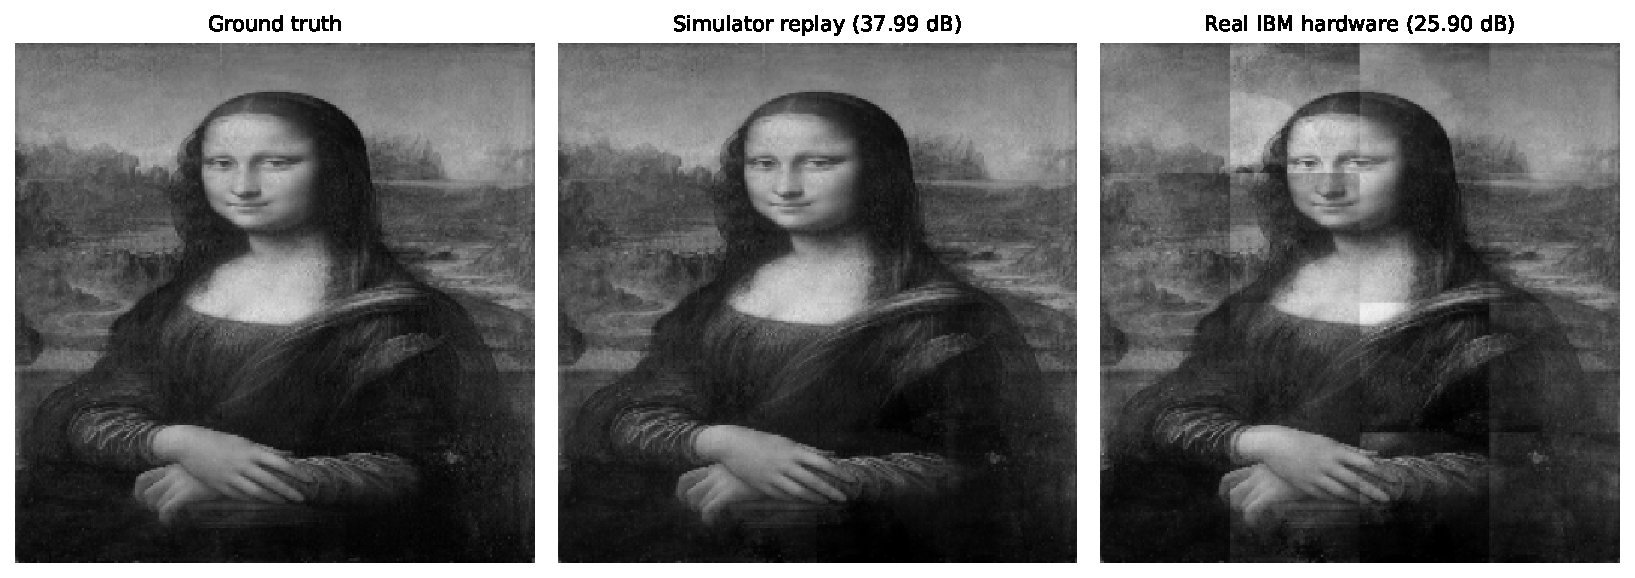
\includegraphics[width=0.85\textwidth]{figures/ibm_hardware_reconstruction_monalisa.pdf}
\caption{\textit{Monalisa} reconstructed from real IBM Quantum hardware measurements (right) against the same trained checkpoint's noiseless-simulator replay (center) and ground truth (left). The hardware image is visibly noisier and exhibits patch-boundary banding, while the subject remains recognizable.}
\label{fig:hardware_reconstruction_monalisa}
\end{figure*}

\begin{figure*}[t]
\centering
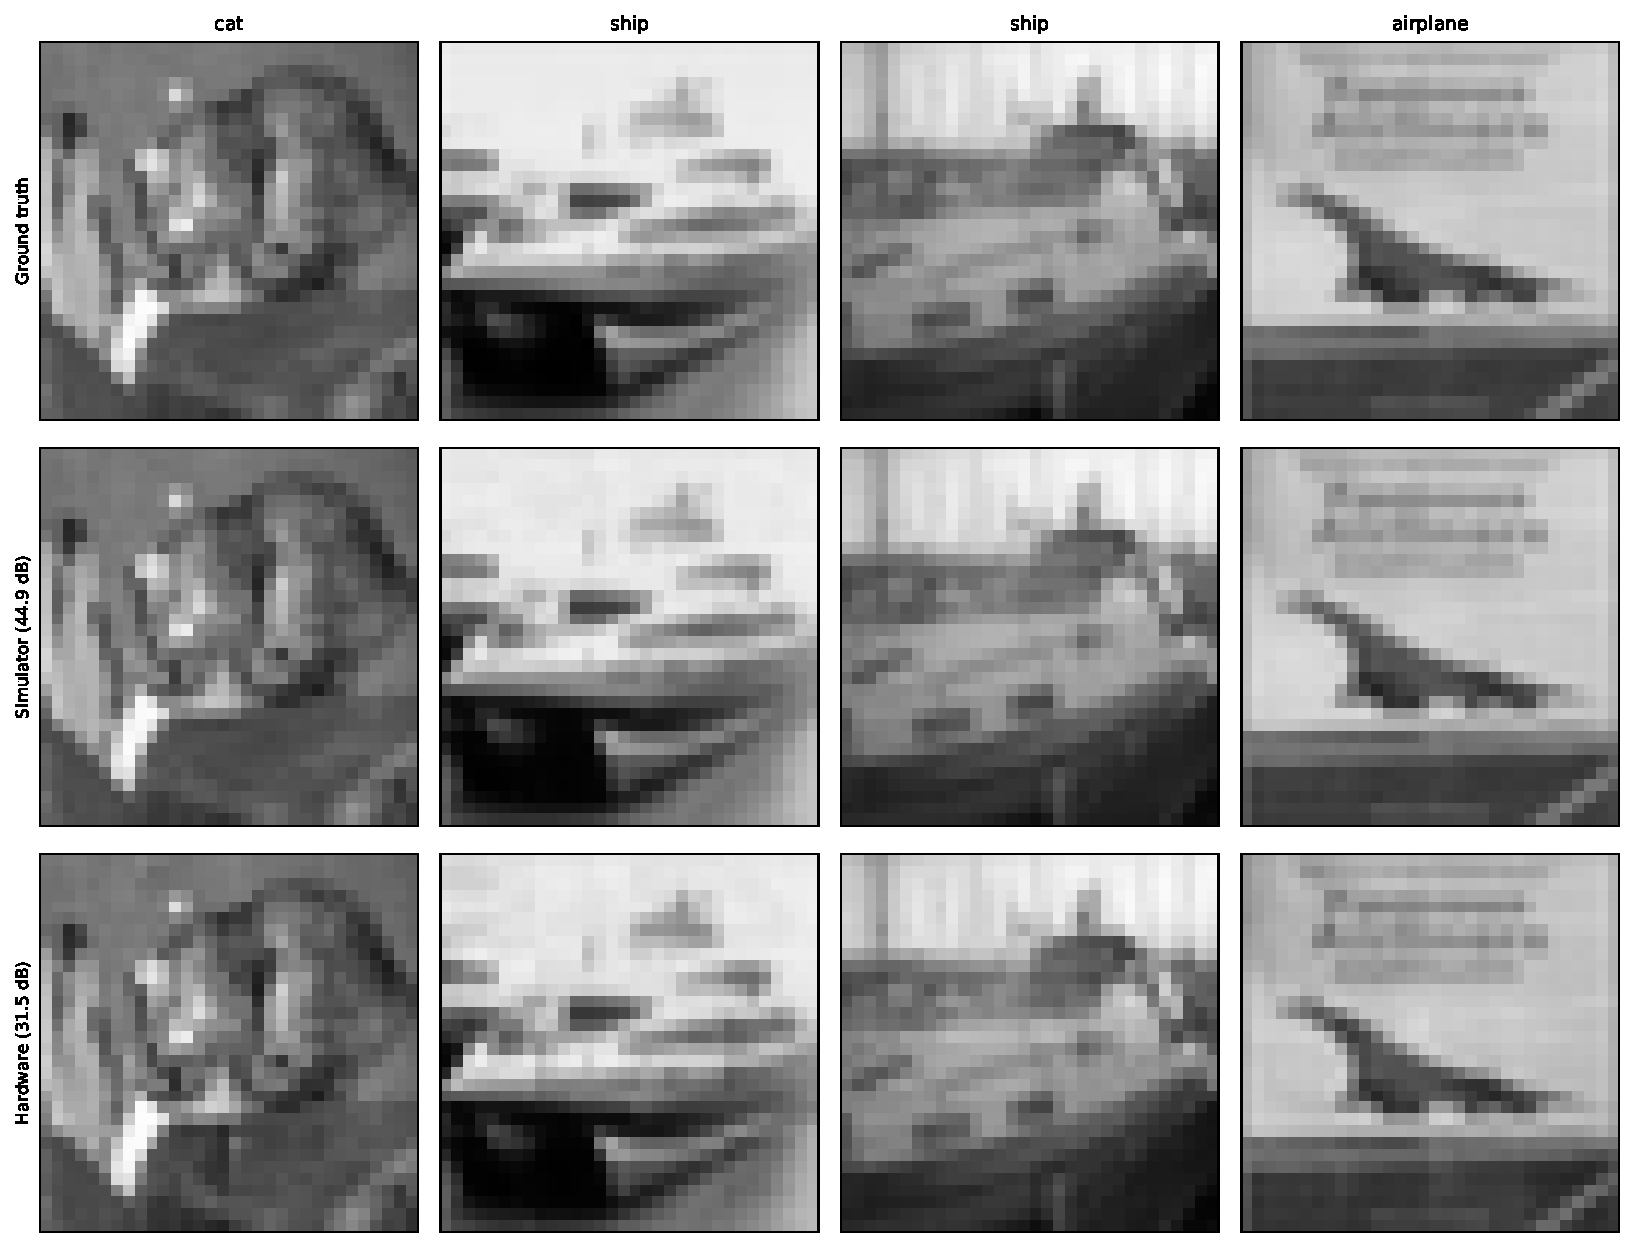
\includegraphics[width=0.85\textwidth]{figures/ibm_hardware_reconstruction_cifar.pdf}
\caption{Four CIFAR-10 images reconstructed from real IBM Quantum hardware measurements (bottom row) against noiseless-simulator replays of the same trained HVK2D checkpoints (middle row) and ground truth (top row).}
\label{fig:hardware_reconstruction_cifar}
\end{figure*}

Five images constitute a pilot, and we make no hardware-advantage claim. The narrower result is that the trained HVK observable channel remains visually and quantitatively informative in these device executions under the reported circuit and shot budget. Full methodology --- exact gate sequences, per-basis measurement construction, job IDs, and pre-submission local-validation results --- is documented in the companion supplementary document.

\subsection{Training-Dynamics Checkpoints Across System Sizes, Replayed on Real Hardware}
\label{sec:checkpoint_hardware_finite_size}
The finite-size comparison of Section~\ref{sec:finite_size_phase_transition} is a noiseless-simulator result. Using the same gate-for-gate checkpoint-replay methodology validated in Section~\ref{sec:hardware_pilot}, we extend it with a genuinely real-hardware complement: we trained fresh HVK1D checkpoints at $N\in\{4,6,8\}$ on two images (\textit{Monalisa}, CIFAR-10 \textit{cat}) for 200 real gradient-descent epochs, saved each checkpoint's exact learned parameters at eight epoch labels ($0,5,10,25,50,100,150,200$, matching the labels used elsewhere in this study), rebuilt each checkpoint's circuit for one representative patch, and executed all $48$ resulting circuits ($2$ images $\times$ $3$ system sizes $\times$ $8$ epoch labels) on \texttt{ibm\_fez} at $256$, $512$, and $1024$ shots. This is a single-patch, single-seed probe --- a lighter circuit budget than the full multi-patch reconstruction pilot above --- so it is a hardware-validation complement to Section~\ref{sec:finite_size_phase_transition}'s multi-seed simulator study, not a replacement for it: real device noise and single-patch/single-seed variance are both present in every point.

\begin{figure}[t]
\centering
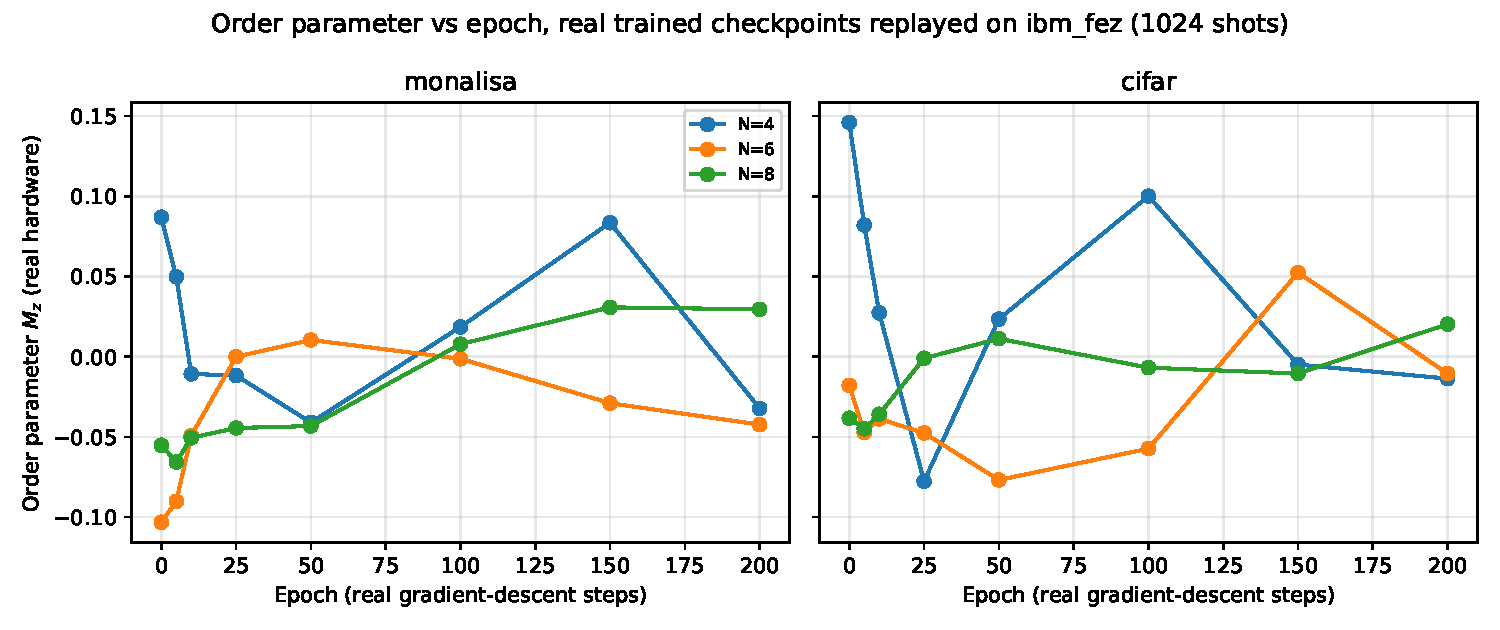
\includegraphics[width=\linewidth]{figures/checkpoint_hardware_order_parameter.pdf}
\caption{Order parameter $M_z(t)$ vs epoch from real trained HVK1D checkpoints ($N=4,6,8$), circuits rebuilt gate-for-gate and executed on real IBM Quantum hardware (\texttt{ibm\_fez}, 1024 shots), one representative patch per image.}
\label{fig:checkpoint_hardware_order_parameter}
\end{figure}

Figure~\ref{fig:checkpoint_hardware_order_parameter} shows the resulting curves are noisier and less structured than their noiseless-simulator counterparts in Figure~\ref{fig:finite_size_phase_transition}, as expected from single-shot-budget hardware measurement of a single patch rather than a change-magnitude trace averaged over multiple images and seeds. We do not apply the descriptive detection rule to these single-patch hardware traces; the figure establishes executable, non-degenerate hardware measurements across epochs, not independent confirmation of the detected change epochs in Table~\ref{tab:finite_size_phase_transition}. The same checkpoints were replayed on the IonQ simulator at the same three shot budgets (Section~\ref{sec:ionq_simulator}); full per-shot data are archived alongside this submission.

\subsection{Cross-Platform Replay on the IonQ Cloud Simulator}
\label{sec:ionq_simulator}
To test software-stack portability separately from device noise, we submitted the same checkpoint circuits through Qiskit to IonQ Quantum Cloud's ideal simulator (\texttt{ionq\_simulator}), with no hardware noise model enabled \cite{IonQBackends}. At each of 256, 512, and 1024 shots, one job contained 48 circuits spanning two images, $N\in\{4,6,8\}$, and eight epochs. All circuits completed, and the mean absolute $M_z$ deviation from the independently sampled 1024-shot trace decreased from $0.0257$ (256 shots) to $0.0213$ (512 shots). A separate 48-circuit, three-basis job reproduced the decreasing $R_{ES}(t)$ shape at 1024 shots.

\begin{figure}[t]
\centering
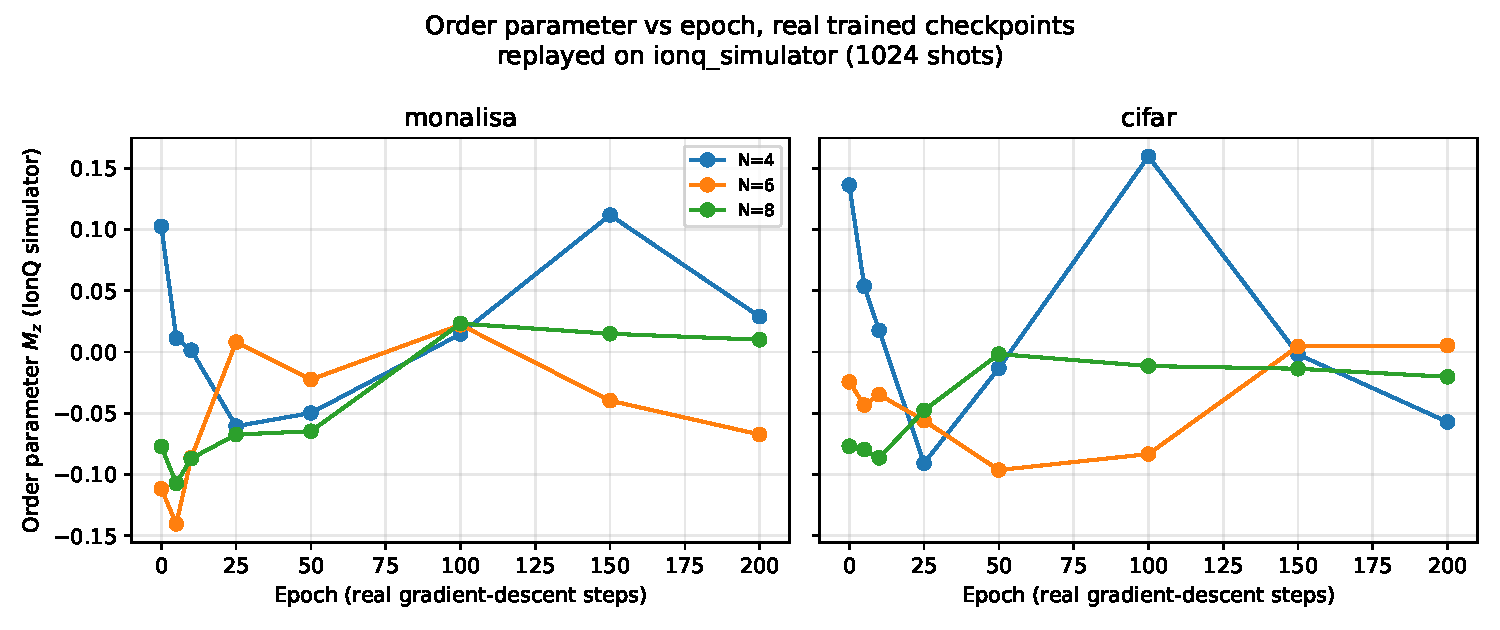
\includegraphics[width=\linewidth]{figures/checkpoint_ionq_order_parameter.pdf}
\caption{Order parameter $M_z(t)$ vs epoch from the same real trained HVK1D checkpoints as Figure~\ref{fig:checkpoint_hardware_order_parameter} ($N=4,6,8$), replayed on the IonQ ideal cloud simulator (\texttt{ionq\_simulator}, 1024 shots) instead of real IBM hardware.}
\label{fig:checkpoint_ionq_order_parameter}
\end{figure}

Figure~\ref{fig:checkpoint_ionq_order_parameter} shows this simulator trace directly, rather than only the summary deviation statistics above: a noiseless, shot-sampling-only analogue of Figure~\ref{fig:checkpoint_hardware_order_parameter}'s hardware traces, same checkpoints and circuits, no device noise. As above, we do not apply the descriptive detection rule of Eq.~\ref{eq:critical_epoch} to these single-patch traces. This is an ideal cloud-simulator portability check, not an IonQ-QPU result; job identifiers, estimator details, and per-circuit summaries are reported in the supplement. The corresponding IonQ $R_{ES}(t)$ replay is shown alongside its own hardware counterpart in Section~\ref{sec:checkpoint_hardware_energy_entanglement}.

\subsection{Noise/Shot Trade-off: A Free Simulator Complement}
\label{sec:hardware_robustness}
The five-image pilot above used a single shot budget (256/basis) and one execution per image, which bounds how much it can say about noise sensitivity on its own. Real IBM Quantum time is a scarce free-tier resource, so we separate what a \emph{calibrated device-noise simulation} can establish at zero hardware cost from what genuinely requires hardware. Using \texttt{qiskit-aer} with the live calibration snapshot of \texttt{ibm\_fez} (\texttt{FakeFez}, no quantum-processor time consumed), we replay the same already-trained checkpoints' circuits at four shot budgets (256/512/1024/4096 shots per basis, three repeated executions each) and compare against both the noiseless-simulator ceiling and the real-hardware point already reported above.

\begin{figure}[t]
\centering
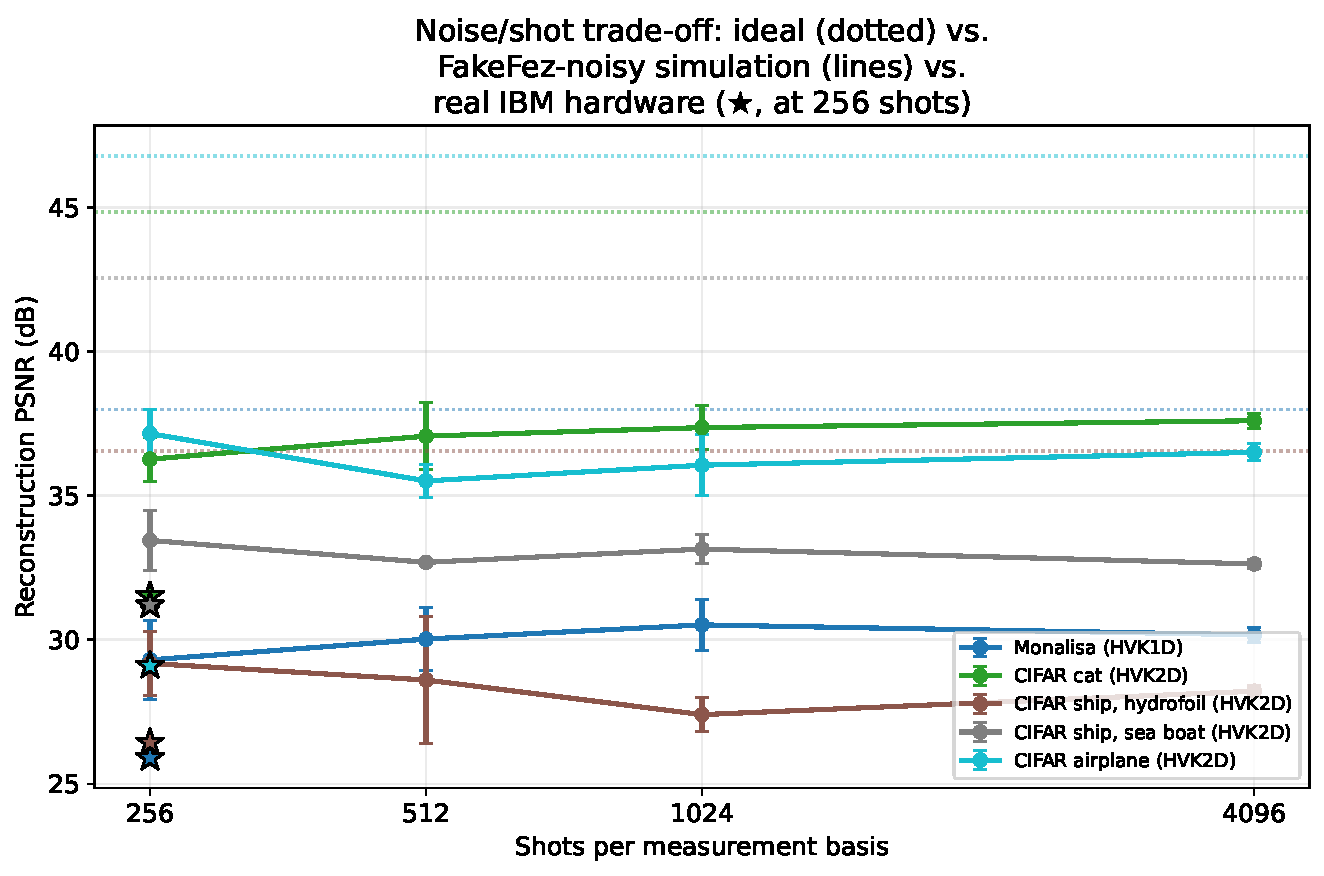
\includegraphics[width=\linewidth]{figures/hardware_robustness_shot_sweep.pdf}
\caption{Calibrated device-noise simulation (\texttt{FakeFez}, mean $\pm$ std over three executions). Dotted lines show noiseless ceilings and stars show real-hardware measurements. Increasing 256 to 4096 shots changes mean PSNR by only $-0.05$~dB.}
\label{fig:hardware_robustness_shot_sweep}
\end{figure}

Two findings follow, averaged over the five checkpoints. First, shot noise accounts for only part of the noiseless-to-real gap: moving from the noiseless ceiling to a calibrated-noise simulation at the same 256-shot budget already costs $8.68$~dB on average, before any real device is involved. Second, more shots does not reliably recover it: increasing to 4096 shots per basis changes PSNR by only $-0.05$~dB on average across the five checkpoints, with individual images ranging from a $1.33$~dB gain to a $0.96$~dB loss --- at this circuit size and shot range, shot count is not a lever that reliably improves reconstruction quality. Comparing the 256-shot noisy simulation directly against the real-hardware point isolates what the calibration snapshot does \emph{not} capture: a further $4.24$~dB average gap (range $2.25$--$8.06$~dB across images), attributable to device effects a single calibration snapshot does not fully capture --- drift between calibration and execution, crosstalk, and correlated errors chief among them. The airplane image is the clear outlier ($8.06$~dB residual gap, roughly double any other image), which we report rather than exclude; a single-execution, five-image pilot cannot distinguish an image-specific effect from ordinary job-to-job variation. This calibrated-noise simulation is a free, repeatable complement to the pilot, not a substitute for it: it bounds how much of the observed hardware gap is attributable to modeled device noise versus unmodeled effects, using zero additional quantum-processor time.

\subsection{Real-Hardware Anchor Points: Repeated Execution and a Second Backend}
\label{sec:hardware_anchors}
The simulated trade-off above is bounded, in turn, by whether it actually reflects real devices. We spent a small, explicitly quota-tracked slice of the free-tier IBM Quantum allowance (four jobs, well under $1\%$ of the monthly limit) confirming it directly: the same two checkpoints (\textit{Monalisa}, CIFAR \textit{cat}) replayed with no retraining on \texttt{ibm\_marrakesh} and \texttt{ibm\_kingston} --- two backends distinct from the original pilot's \texttt{ibm\_fez} --- at the original 256-shot budget and, separately, at 1024 shots.

\begin{table}[t]
\centering
\caption{Real-hardware anchor points: same checkpoints, no retraining, on two further backends. The original pilot's \texttt{ibm\_fez} point is shown for reference.}
\label{tab:hardware_anchors}
\scriptsize
\begin{tabular}{lccc}
\toprule
Image & Backend & Shots & PSNR (dB) \\
\midrule
Monalisa & ibm\_fez (original pilot) & 256 & 25.90 \\
Monalisa & ibm\_marrakesh & 256 & 25.94 \\
Monalisa & ibm\_kingston & 1024 & 26.10 \\
CIFAR cat & ibm\_fez (original pilot) & 256 & 31.52 \\
CIFAR cat & ibm\_kingston & 256 & 28.93 \\
CIFAR cat & ibm\_kingston & 1024 & 31.24 \\
\bottomrule
\end{tabular}
\end{table}

\textit{Monalisa} reproduces almost exactly across backends at matched shots ($25.94$ vs.\ $25.90$~dB, \texttt{ibm\_marrakesh} vs.\ \texttt{ibm\_fez}), and gains only $0.16$~dB from quadrupling shots to 1024 --- consistent with the simulated finding above that shot count is not a reliable lever. The CIFAR \textit{cat} point is the more informative one: on \texttt{ibm\_kingston} at the original 256-shot budget it reaches $28.93$~dB, $2.59$~dB below the \texttt{ibm\_fez} pilot point, while its own 1024-shot execution on the same backend recovers to $31.24$~dB, within $0.28$~dB of the original. This is real job-to-job and backend-to-backend variation of a magnitude comparable to the unmodeled residual identified by the simulator comparison (Section~\ref{sec:hardware_robustness}) --- direct evidence, not merely a simulated bound, that a single 256-shot execution on a single backend is not yet a stable estimate of this pipeline's hardware performance, and that repeated execution matters at least as much as backend choice or shot count individually.

\subsection{Provable \texorpdfstring{$D_4$}{D4} Symmetry}
\label{sec:d4}
\label{sec:symmetry}
A $D_4$-pooled HVK2D observable-grid map is equivariant to the eight symmetries of the square \emph{by construction}: $\Phi_{D_4}(x)=\frac{1}{8}\sum_{g\in D_4}P_g^{-1}\Phi(gx)$ averages the unpooled map over the group orbit, so $\Phi_{D_4}(hx)=P_h\Phi_{D_4}(x)$ for every $h\in D_4$ up to floating-point error. We verify this numerically over 7000 patch transforms of cached CIFAR images (Table~\ref{tab:d4_equivariance}, Figure~\ref{fig:d4_equivariance}): the pooled map's equivariance error is $9.57\times10^{-17}\pm1.26\times10^{-17}$ (floating-point noise), while the original unpooled positional map is not measurably more symmetric than a local/raw control ($0.815\pm0.129$ vs.\ $0.837\pm0.131$) --- confirming the unpooled map is only $D_4$-\emph{motivated} by the patch grid's geometry, not empirically equivariant, and that only the explicit pooling construction delivers the property. This is currently a feature-grid-level construction and numerical diagnostic rather than a component of the trainable reconstruction pipeline; integrating it end-to-end (Section~\ref{sec:limitations}) is concrete future work.

\begin{table}[t]
\centering
\caption{$D_4$ equivariance error for unpooled and pooled observable-grid maps (lower is better; pooled map is group-averaged over all eight square symmetries).}
\label{tab:d4_equivariance}
\scriptsize
\begin{tabular}{l@{\hspace{2em}}c@{\hspace{2em}}c}
\toprule
Model & Mean error & Std. error \\
\midrule
$D_4$-pooled HVK2D & $9.57\times10^{-17}$ & $1.26\times10^{-17}$ \\
No positional encoding & $7.40\times10^{-1}$ & $1.52\times10^{-1}$ \\
HVK2D positional & $8.15\times10^{-1}$ & $1.29\times10^{-1}$ \\
Local/raw & $8.37\times10^{-1}$ & $1.31\times10^{-1}$ \\
\bottomrule
\end{tabular}
\end{table}

\begin{figure}[t]
\centering
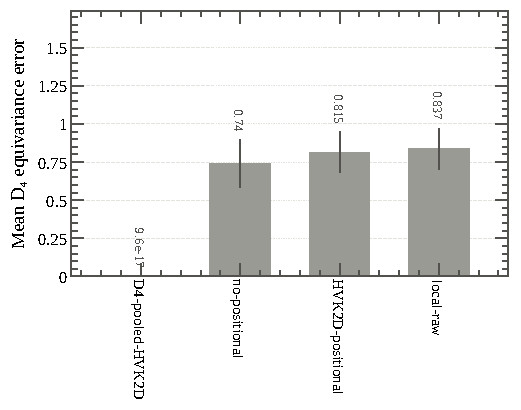
\includegraphics[width=\linewidth]{figures/d4_equivariance_summary.pdf}
\caption{$D_4$ equivariance diagnostic. The unpooled positional map is not equivariant; the group-pooled map is equivariant to numerical precision.}
\label{fig:d4_equivariance}
\end{figure}

\subsection{Entanglement Necessity in the Nonlocal-Structure Protocol}
\label{sec:entanglement_necessity}
This diagnostic is deliberately constructed to reward pair-observable structure: the target is a fixed synthetic function of \emph{simulated} patch features not concatenated into any candidate's own input block (the companion supplement gives the leakage-audit procedure that rules out circularity), and every control receives the same raw inputs as HVK2D. Table~\ref{tab:hvk_pair_diagnostic} and Figure~\ref{fig:hvk_pair_diagnostic} report the result across five seeds: HVK2D's entangling observable channel reaches mean $R^2=0.9735$ ($32.77$~dB PSNR), a $17.74$~dB improvement over a no-entanglement control ($R^2=0.019$) and $18.52$~dB over random-VQC latents ($R^2=-0.173$); freezing the quantum circuit (features fixed, only readout trained) still reaches $R^2=0.853$, while a parameter-matched classical control ($R^2=-0.030$) and a frozen-classical control ($R^2=-0.903$) fail outright. This is evidence that an entangling pair-observable channel is \emph{representationally necessary within the tested feature class and fixed linear-readout protocol} to fit this target.

\begin{table*}[t]
\centering
\caption{HVK2D restricted pair-correlation diagnostic across five seeds. Deliberately favorable to pair-observable structure; evidence for entanglement-necessity under a matched linear readout.}
\label{tab:hvk_pair_diagnostic}
\scriptsize
\begin{tabular}{lccc}
\toprule
Model & Mean MSE & Mean PSNR (dB) & Mean $R^2$ \\
\midrule
HVK2D entangling observables & $8.5969\times10^{-4}$ & 32.77 & 0.9735 \\
Freeze quantum & $4.7904\times10^{-3}$ & 27.34 & 0.8533 \\
No entanglement & $3.1461\times10^{-2}$ & 15.03 & 0.0191 \\
Raw-linear classical & $3.1654\times10^{-2}$ & 15.00 & 0.0133 \\
Parameter-matched classical & $3.3033\times10^{-2}$ & 14.82 & $-0.0297$ \\
Random VQC & $3.7616\times10^{-2}$ & 14.25 & $-0.1732$ \\
Freeze classical & $6.0973\times10^{-2}$ & 12.17 & $-0.9025$ \\
\bottomrule
\end{tabular}
\end{table*}

\begin{figure*}[t]
\centering
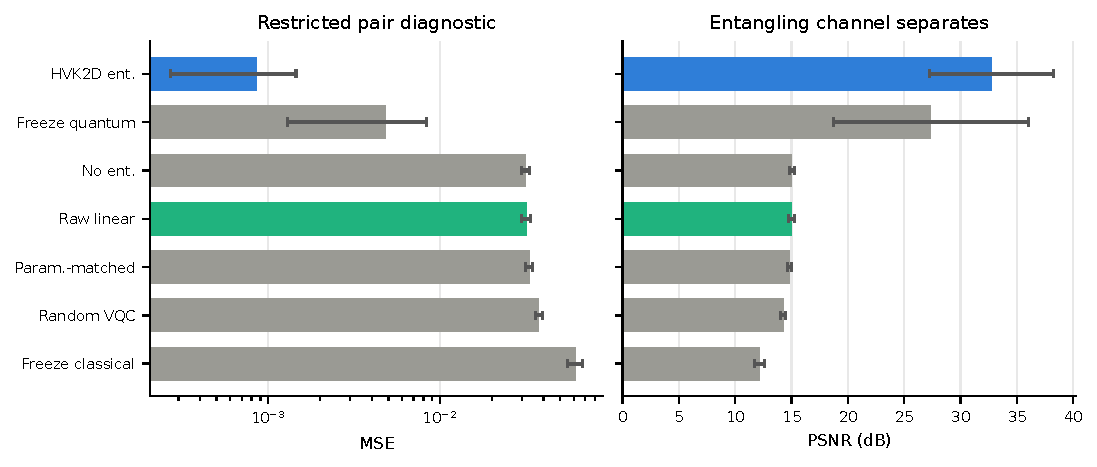
\includegraphics[width=0.78\textwidth]{figures/full_ablation_metric_comparison.pdf}
\caption{Restricted pair-correlation diagnostic summary (mean $\pm$ std over five seeds). The entangling observable feature map dominates every control on this deliberately favorable task.}
\label{fig:hvk_pair_diagnostic}
\end{figure*}

\subsection{Training-Dynamics Change-Point Diagnostic: A Corrected Multi-Seed Result}
\label{sec:phase_transition}
We test for abrupt changes in the learned representation during optimization. This is an exploratory change-point diagnostic on a magnetization-style summary, not a thermodynamic phase transition, a singularity, or an infinite-system claim. An earlier version was withdrawn after a provenance audit: the restricted-diagnostic trajectories previously shown were analytic interpolations produced for visualization rather than measurements from saved checkpoints, and the original multi-dataset traces were recorded during training, where HVK2D's training-mode forward pass deliberately adds Gaussian observable noise that confounds parameter evolution with injected jitter. The corrected runner evaluates a separate, noise-free forward pass in evaluation mode immediately after every optimizer update and tracks the resulting global order parameter $M_z(t)$, the mean of the $N$ local-$Z$ observables over all $P$ patches at optimizer step (epoch) $t$:
\begin{equation}
M_z(t) = \frac{1}{P N}\sum_{p=1}^{P}\sum_{i=1}^{N}\langle Z_i\rangle_p(t).
\label{eq:order_parameter}
\end{equation}
Detection uses the change magnitude $\mathcal{X}(t)=|M_z(t)-M_z(t-\Delta t)|$ (identically defined on $R_{ES}(t)$ in place of $M_z(t)$ for the energy-to-entanglement-ratio diagnostic of Section~\ref{sec:critical_temperature}), a per-run adaptive threshold $\theta$, and a detected change epoch $t_c$:
\begin{align}
\theta &= \operatorname{median}_t\big(\mathcal{X}(t)\big) + 2\operatorname{std}_t\big(\mathcal{X}(t)\big), \\
t_c &= \begin{cases}
\displaystyle\operatorname*{arg\,max}_t \mathcal{X}(t) & \text{if } \max_t \mathcal{X}(t) > \theta > 0, \\
\text{not detected} & \text{otherwise.}
\end{cases}
\label{eq:critical_epoch}
\end{align}
The threshold is computed per run from that run's own trace; it is not a fixed global constant or a null-calibrated statistical test. Thus ``detected'' means only that a run's sharpest observed change exceeds this descriptive within-run threshold. It does not supply a $p$-value, control a false-positive rate, or establish a physical transition.

Table~\ref{tab:phase_transition_corrected} reports the result across all six datasets (two images $\times$ two seeds each, 24 runs total). Detection is not universal: MNIST triggers in all four runs, BloodMNIST and PneumoniaMNIST in three of four, and CIFAR-10, Fashion-MNIST, and PathMNIST in two of four, for an overall descriptive rate of $16/24$ ($66.7\%$). Because the threshold is selected from the same trajectory it evaluates and the sample contains only two seeds per image, these rates are exploratory summaries rather than inferential evidence for dataset-specific transition probabilities.

\begin{table}[t]
\centering
\caption{Corrected, noise-free training-dynamics diagnostic across all six datasets (2 images $\times$ 2 seeds/dataset).}
\label{tab:phase_transition_corrected}
\scriptsize
\begin{tabular}{lcccc}
\toprule
Dataset & $n$ & Detected & Mean $t_c$ & Mean $\mathcal{X}_{\max}$ \\
\midrule
CIFAR-10 & 4 & 2/4 & 64.0 & $0.0036\pm0.0009$ \\
MNIST & 4 & 4/4 & 98.75 & $0.0023\pm0.0012$ \\
Fashion-MNIST & 4 & 2/4 & 45.0 & $0.0027\pm0.0011$ \\
PathMNIST & 4 & 2/4 & 54.5 & $0.0038\pm0.0015$ \\
BloodMNIST & 4 & 3/4 & 96.0 & $0.0033\pm0.0012$ \\
PneumoniaMNIST & 4 & 3/4 & 103.0 & $0.0036\pm0.0008$ \\
\midrule
Total & 24 & $16/24$ & -- & -- \\
\bottomrule
\end{tabular}
\end{table}

\subsection{System-Size Sensitivity of the Detected Change Epoch}
\label{sec:finite_size_phase_transition}
Every result above is measured at a single, fixed system size (HVK2D's six-qubit grid). We therefore ask whether the descriptive change epoch depends on circuit width. HVK2D's grid topology is fixed at six qubits by construction, so this comparison uses HVK1D's parameterized chain topology. We reran the corrected protocol from Section~\ref{sec:phase_transition} at $N=4$, $N=6$, and $N=8$ qubits on two datasets (CIFAR-10 and MNIST), one image and two seeds each (four runs per size, 200 epochs). Three sizes and four runs per size are insufficient for finite-size scaling or critical-exponent analysis; the experiment is a sensitivity check on the diagnostic only.

All twelve runs register a detection under the same threshold rule (Table~\ref{tab:finite_size_phase_transition}), but the detected epoch is not monotonic in $N$: $10.0\pm12.7$ at $N=4$, $85.0\pm50.1$ at $N=6$, and $61.0\pm65.2$ at $N=8$. Three of the four $N=8$ traces stay near $M_z\approx0$ and trigger on small early changes, whereas one MNIST run develops a late excursion at $t_c=172$ that dominates the variance. The result therefore shows instability of this heuristic across width and initialization, not a scaling law or evidence of a critical point.

\begin{table}[t]
\centering
\caption{Finite-size comparison of the order-parameter diagnostic, HVK1D, CIFAR-10 + MNIST (1 image $\times$ 2 seeds per dataset per $N$).}
\label{tab:finite_size_phase_transition}
\scriptsize
\begin{tabular}{lcccc}
\toprule
$N$ (qubits) & $n$ & Detected & Mean $t_c$ & Std $t_c$ \\
\midrule
4 & 4 & 4/4 & 10.0 & 12.7 \\
6 & 4 & 4/4 & 85.0 & 50.1 \\
8 & 4 & 4/4 & 61.0 & 65.2 \\
\bottomrule
\end{tabular}
\end{table}

\begin{figure}[t]
\centering
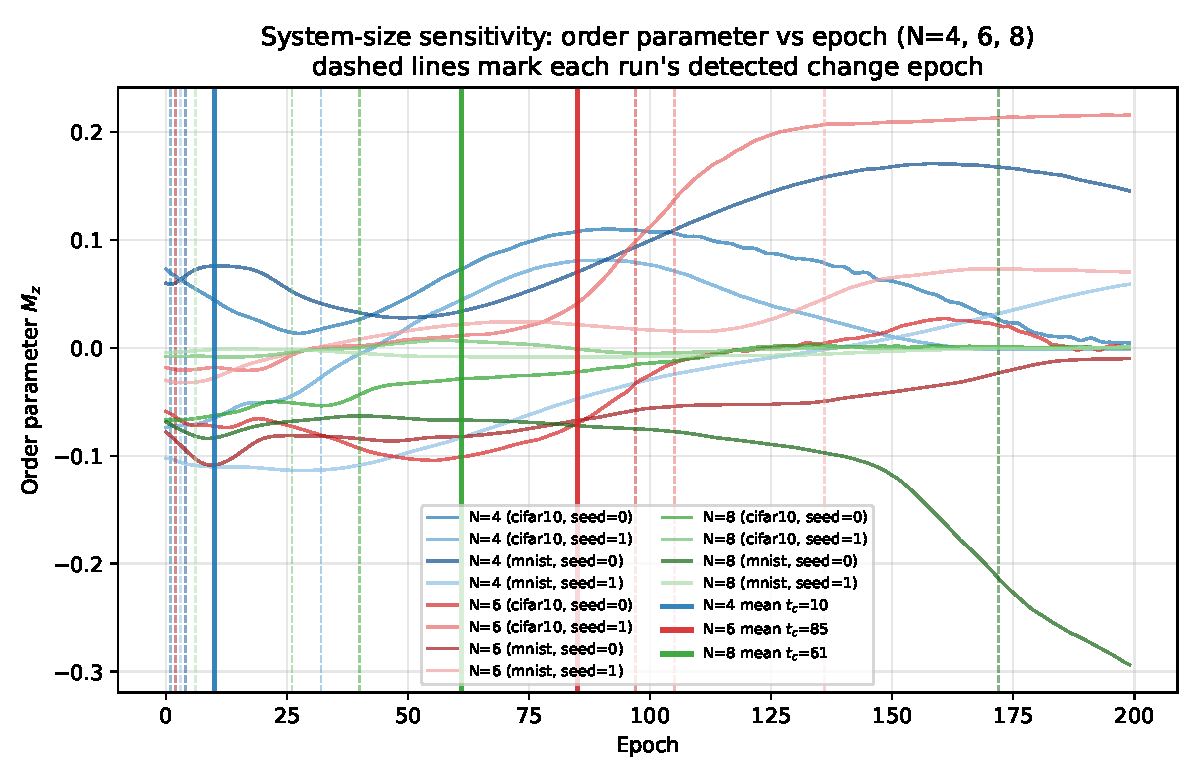
\includegraphics[width=\linewidth]{figures/finite_size_phase_transition.pdf}
\caption{Order parameter $M_z(t)$ vs epoch, HVK1D, $N=4$ (blue), $N=6$ (red), and $N=8$ (green), four runs each. Dashed lines mark within-run detected change epochs; solid lines mark per-$N$ means. Most $N=8$ traces stay near zero, while one late outlier drives much of the variance.}
\label{fig:finite_size_phase_transition}
\end{figure}

Table~\ref{tab:finite_size_phase_transition} summarizes per-run detections: each run's own change magnitude is thresholded independently, then the resulting change epochs are averaged, giving a non-monotonic mean ($10.0\to85.0\to61.0$). A complementary view averages the change-magnitude \emph{traces themselves} across the four runs at each $N$ before locating a peak, rather than averaging four independently-detected peak locations. This ensemble-mean view (Figure~\ref{fig:finite_size_mean_susceptibility}) shows the peak of $\langle|\Delta M_z(t)|\rangle$ shifting later with $N$: epoch $3$ at $N=4$, epoch $96$ at $N=6$, epoch $163$ at $N=8$ --- monotonic, in contrast to Table~\ref{tab:finite_size_phase_transition}. We report both because they are not the same statistic and can disagree: per-run thresholding is sensitive to whichever single epoch happens to cross that run's own noisy threshold, while the ensemble mean suppresses run-to-run idiosyncrasy at the cost of blurring together events that do not align in time across runs. The $N=4$ peak at epoch $3$ sits at the very start of training, where curves are dominated by initialization transients rather than a mid-training reorganization, and should be read with that caveat; $N=6$ produces the sharpest, best-separated peak of the three (Figure~\ref{fig:finite_size_mean_susceptibility}), while $N=8$'s peak is broad and comparable in height to its own baseline fluctuation. With four runs per $N$, the shaded $\pm$one-std bands in Figure~\ref{fig:finite_size_mean_susceptibility} are wide enough that we treat the monotonic peak-shift as a second exploratory observation alongside Table~\ref{tab:finite_size_phase_transition}'s non-monotonic one, not as a resolution of it.

\begin{figure}[t]
\centering
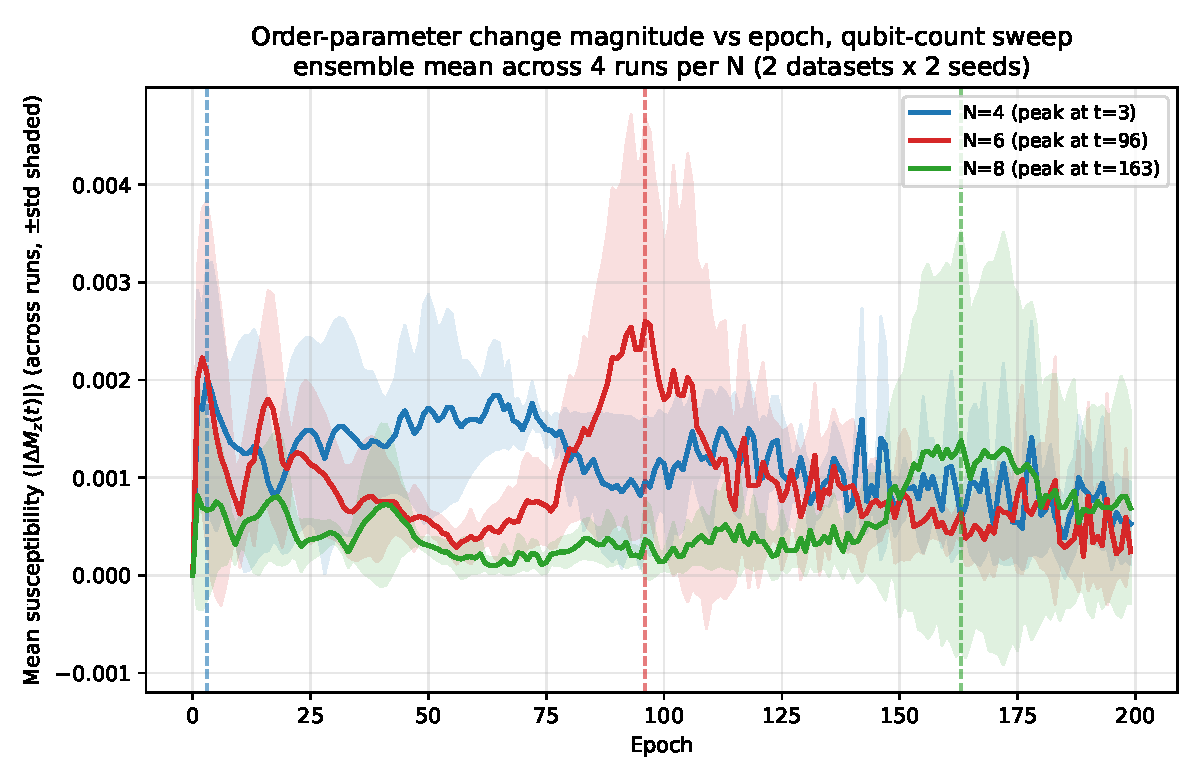
\includegraphics[width=\linewidth]{figures/finite_size_mean_susceptibility.pdf}
\caption{Ensemble-mean change magnitude $\langle|\Delta M_z(t)|\rangle$ vs epoch, averaged across the four runs at each $N$ before peak-finding (shaded: $\pm$one std across runs), $N=4$ (blue), $N=6$ (red), $N=8$ (green). Dashed vertical lines mark each curve's peak epoch. The peak shifts monotonically later with $N$ (epochs $3$, $96$, $163$), a different statistic from the per-run-averaged epochs in Table~\ref{tab:finite_size_phase_transition}.}
\label{fig:finite_size_mean_susceptibility}
\end{figure}

\subsection{A Second, Orthogonal Size Axis: MPS Bond Dimension}
\label{sec:bond_dimension_phase_transition}
Qubit count $N$ is a quantum circuit-width parameter; a second, purely classical size parameter enters before the circuit. We test whether the detected change epoch depends on MPS compression fidelity, holding $N=6$ fixed and varying $\chi\in\{1,2,4,8\}$ on CIFAR-10 (\textit{cat}), with two seeds each.

All eight runs trigger, but the two seeds disagree sharply at $\chi=1$ and $\chi=2$ and agree closely at $\chi=4$ and $\chi=8$. The trajectories separate into qualitatively different optimization paths at low $\chi$ and similar rising paths at higher $\chi$. With only two seeds per setting, this is a hypothesis-generating observation that richer compression may reduce initialization sensitivity; it is not sufficient to estimate a population variance trend or establish a general relationship between bond dimension and optimization dynamics.

This is a different measurement from, but worth reading alongside, the companion supplementary study's single-seed finding that MPS bond dimension is non-monotonic for \emph{final reconstruction quality}: under a fixed step budget, $\chi=1$ and $\chi=2$ outperform the default $\chi=4$ on PSNR, with $\chi=8$ only partially recovering. Taken together, the two results suggest bond dimension may trade off \emph{where} training ends up (reconstruction quality) against \emph{how reproducibly it gets there} (seed-to-seed agreement in training dynamics), rather than acting as a simple compression-fidelity knob on either axis --- a connection neither single result establishes on its own.

\begin{table}[t]
\centering
\caption{MPS bond-dimension comparison of the order-parameter diagnostic, HVK1D, $N=6$ fixed, CIFAR-10 cat (2 seeds per $\chi$).}
\label{tab:bond_dimension_phase_transition}
\scriptsize
\begin{tabular}{lcccc}
\toprule
$\chi$ (MPS bond dim.) & $n$ & Detected & Mean $t_c$ & Std $t_c$ \\
\midrule
1 & 2 & 2/2 & 88.5 & 86.5 \\
2 & 2 & 2/2 & 52.0 & 50.0 \\
4 & 2 & 2/2 & 101.0 & 4.0 \\
8 & 2 & 2/2 & 95.0 & 2.0 \\
\bottomrule
\end{tabular}
\end{table}

\begin{figure}[t]
\centering
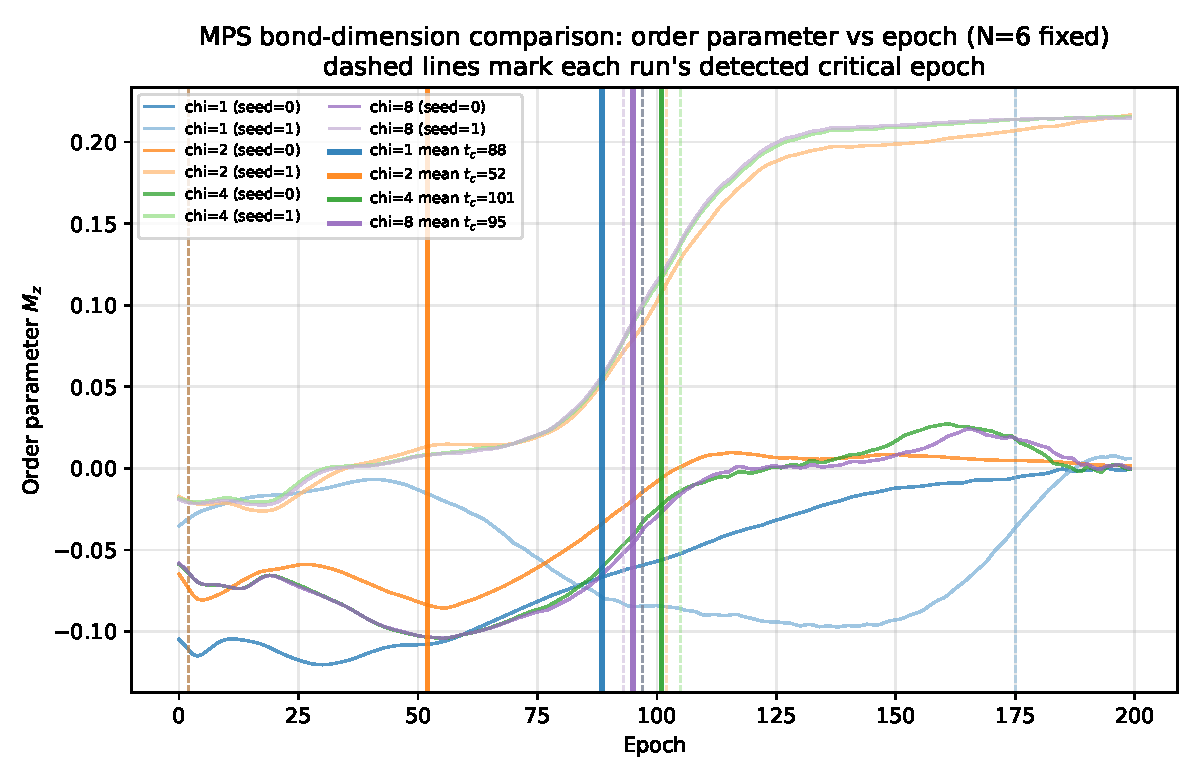
\includegraphics[width=\linewidth]{figures/bond_dimension_phase_transition.pdf}
\caption{Order parameter $M_z(t)$ vs epoch, HVK1D, $N=6$ fixed, MPS bond dimension $\chi\in\{1,2,4,8\}$, two seeds each. Dashed lines mark detected change epochs and solid lines mark per-$\chi$ means. The two-seed patterns are descriptive and not a population-level variance estimate.}
\label{fig:bond_dimension_phase_transition}
\end{figure}

As an execution check, we also replayed trained checkpoints across all four bond dimensions on real \texttt{ibm\_marrakesh} hardware and the IonQ ideal simulator at 256, 512, and 1024 shots. All checkpoint circuits completed and produced non-degenerate order parameters, but the single-patch, single-seed replay cannot confirm the cross-seed pattern above. The companion supplement reports the complete twelve-job audit trail, the hardware curves, and a three-basis $R_{ES}$ replay; it also documents why $\chi=1$ is excluded from the ratio because its product-state entropy reaches the numerical floor.

\subsection{Energy-to-Entanglement Ratio as an Orthogonal Diagnostic}
\label{sec:critical_temperature}
The learned Heisenberg energy provides a second scalar view of training. We define the signed energy-to-entanglement ratio
\begin{align}
R_{ES}(t)&=\frac{H(t)}{S},\\
H(t)&=\sum_i\Bigl[J_x^{(i)}\langle X_iX_{i+1}\rangle
J_y^{(i)}\langle Y_iY_{i+1}\rangle \nonumber\\
&\hspace{3.0em}+J_z^{(i)}\langle Z_iZ_{i+1}\rangle\Bigr].
\end{align}
where $S=\sum_i S_i$ is the fixed sum of von Neumann bond entropies from the classical MPS decomposition. This ratio has units of energy per entropy unit and is \emph{not} a thermodynamic temperature: no Gibbs state is fitted, no derivative $\partial S/\partial E$ is evaluated, and its negative sign reflects the learned signed Hamiltonian. The bond correspondence is clean only for HVK1D at six sites, so we track $R_{ES}(t)$ there on two CIFAR-10 images over four seeds and apply the same descriptive change-threshold rule to $|\Delta R_{ES}(t)|$.

\begin{figure}[t]
\centering
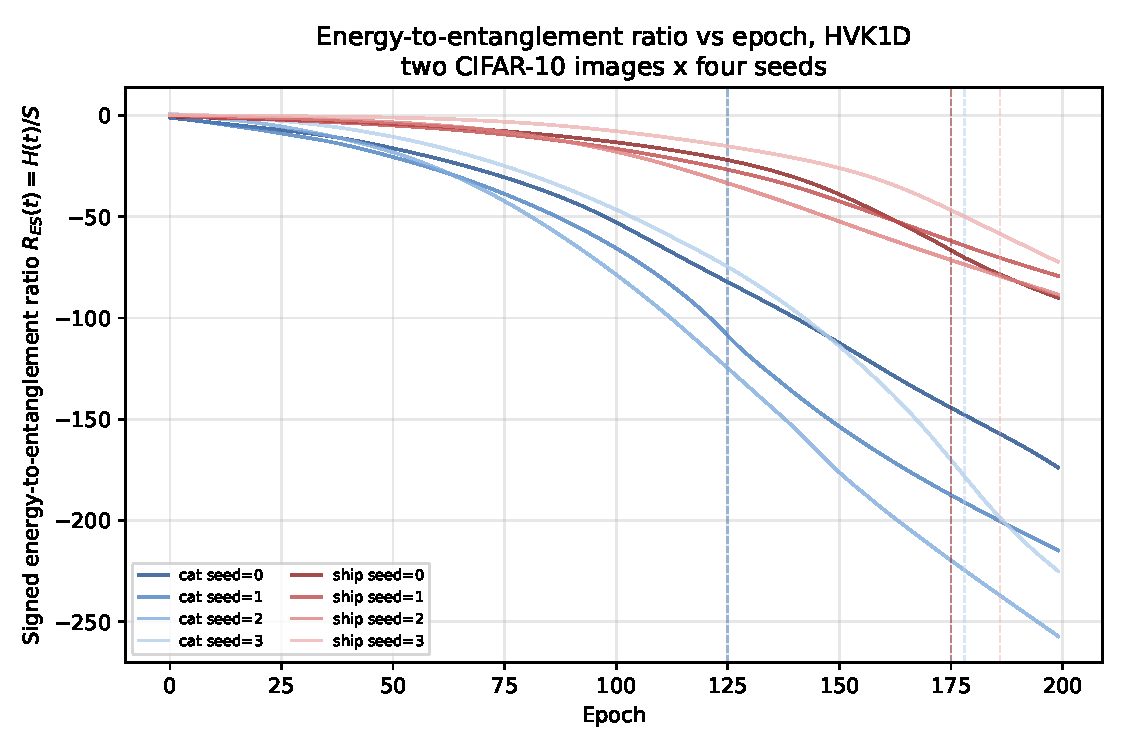
\includegraphics[width=\linewidth]{figures/critical_temperature_traces.pdf}
\caption{Signed energy-to-entanglement ratio $R_{ES}(t)=H(t)/S$ across training, HVK1D, two CIFAR-10 images $\times$ four seeds. The increasingly negative traces reflect the learned signed energy at fixed $S$; they are not temperature or cooling curves.}
\label{fig:critical_temperature}
\end{figure}

\begin{figure}[t]
\centering
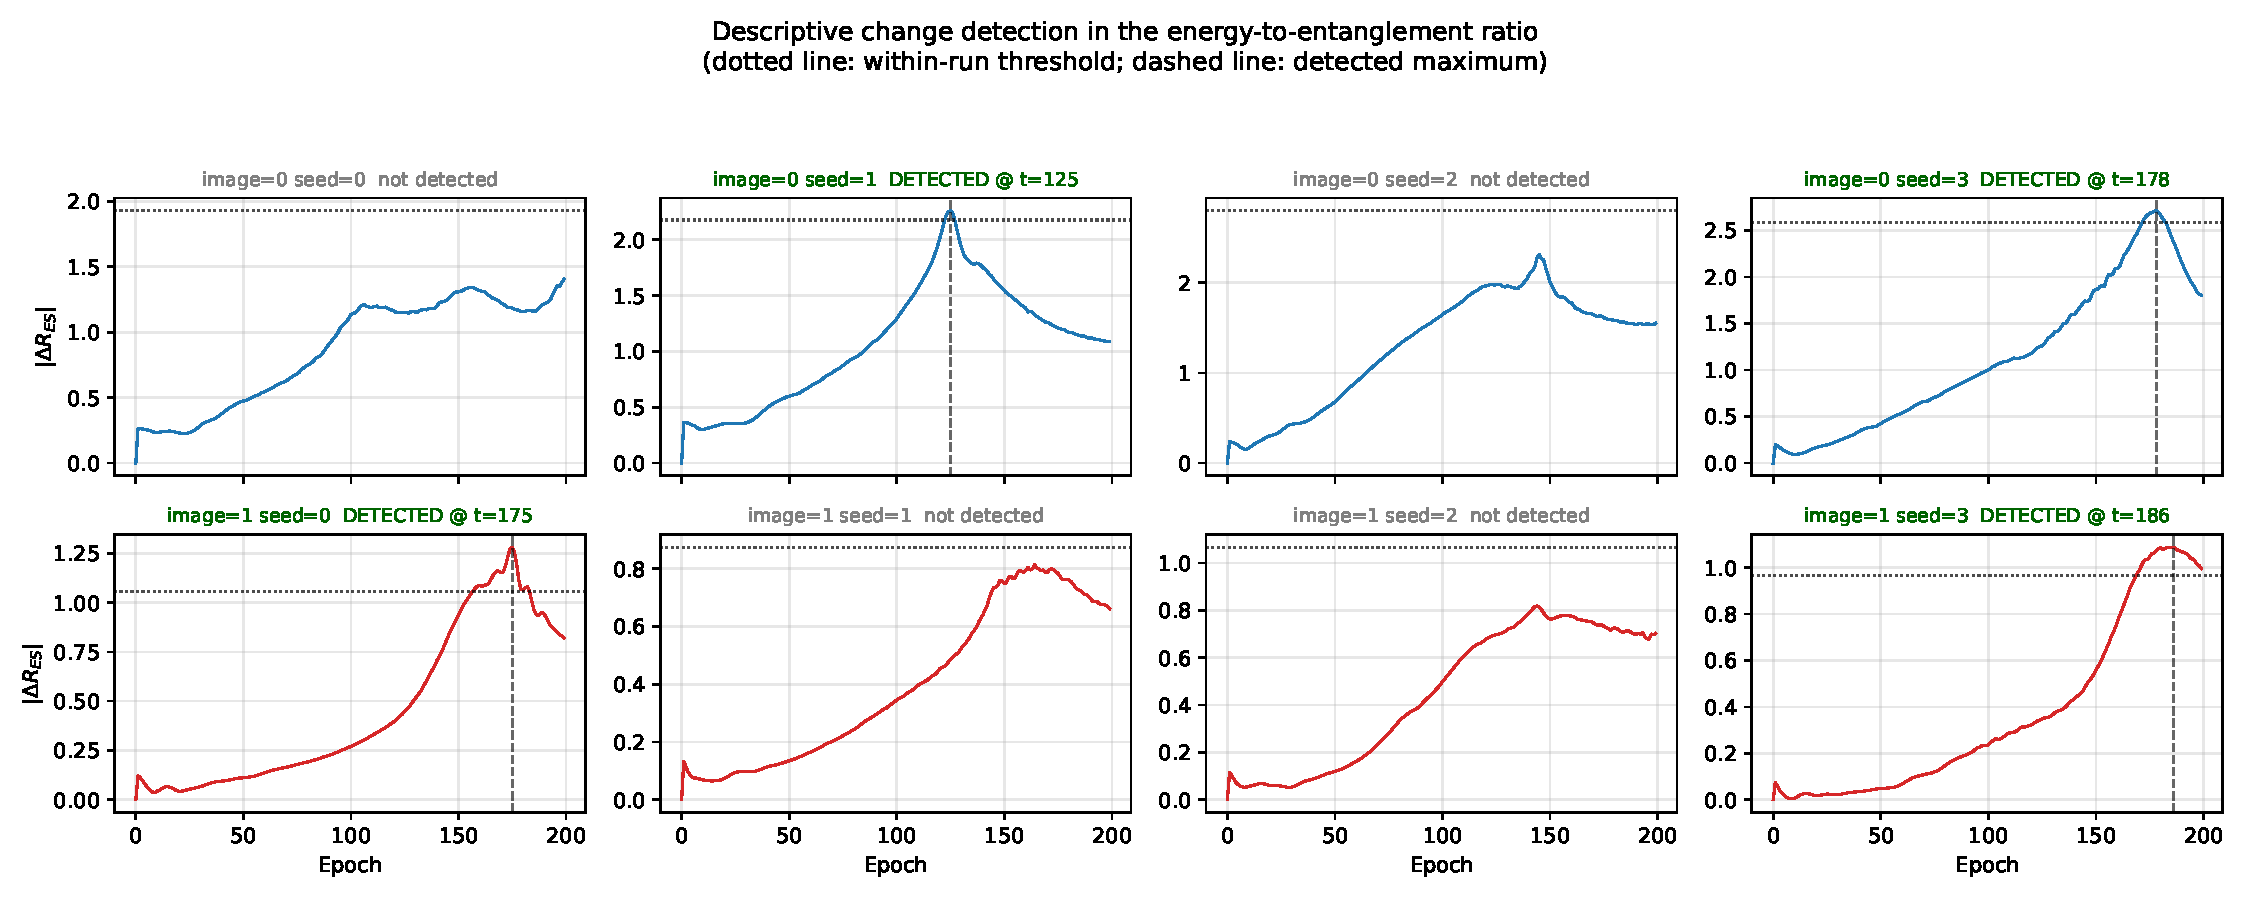
\includegraphics[width=\linewidth]{figures/critical_temperature_susceptibility.pdf}
\caption{Change magnitude $|\Delta R_{ES}(t)|$ vs epoch. The dotted line is the descriptive within-run threshold; a dashed vertical line marks the maximum when it exceeds that threshold.}
\label{fig:critical_temperature_susceptibility}
\end{figure}

All eight $R_{ES}$ traces become more negative as learned signed energy decreases at fixed $S$, and four of eight exceed the descriptive change threshold. Broad peaks occur around epochs 100--180 in every run, but their threshold status depends on within-run scale. The small sample and data-dependent threshold preclude an inferential claim; the result shows only that energy- and magnetization-based summaries can both exhibit nonuniform changes during optimization.

\subsection{Energy-to-Entanglement Ratio, Replayed on Real Hardware}
\label{sec:checkpoint_hardware_energy_entanglement}
Using the same checkpoint-replay methodology as Section~\ref{sec:checkpoint_hardware_finite_size}, we measure $R_{ES}(t)$ itself from real hardware rather than from simulation. The $R_{ES}$ construction requires $N=6$ (Section~\ref{sec:critical_temperature}), so this replay is single-size: we trained fresh HVK1D checkpoints at $N=6$ on the same two images (\textit{Monalisa}, CIFAR-10 \textit{cat}) for 200 real gradient-descent epochs, saved each checkpoint's learned $J_x^{(i)},J_y^{(i)},J_z^{(i)}$ couplings and projected per-qubit angles at the same eight epoch labels, and measured all three Pauli bases needed to reconstruct $\langle X_iX_{i+1}\rangle$, $\langle Y_iY_{i+1}\rangle$, $\langle Z_iZ_{i+1}\rangle$ per bond ($2$ images $\times$ $8$ epoch labels $\times$ $3$ bases $=48$ circuits) on \texttt{ibm\_marrakesh} at $256$, $512$, and $1024$ shots. Hardware-measured bond correlators are combined with each checkpoint's own learned couplings and the fixed, classically-computed bond entropy $S$ to obtain $R_{ES}(t)$; this is a single-patch, single-seed probe, the same limitation noted in Section~\ref{sec:checkpoint_hardware_finite_size}.

As a cross-platform check of the three-basis measurement path, the same 48 circuits were also executed as one 1024-shot job on the IonQ ideal cloud simulator (job identifier retained in the archive). Since this execution used an ideal simulator rather than an IonQ QPU, it supports software-stack portability and estimator reproducibility only.

\begin{figure}[t]
\centering
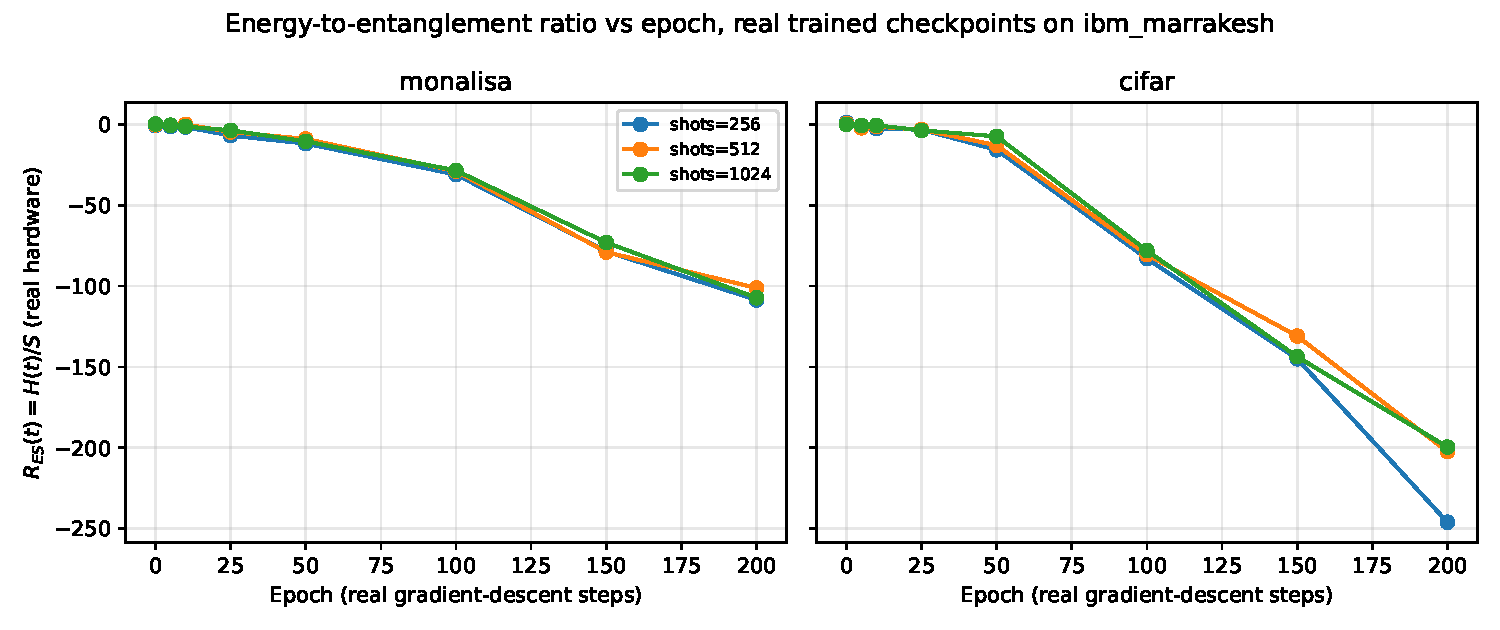
\includegraphics[width=\linewidth]{figures/checkpoint_hardware_energy_entanglement_ratio.pdf}
\caption{$R_{ES}(t)=H(t)/S$ from real trained HVK1D checkpoints ($N=6$), Pauli bond correlators measured on real IBM Quantum hardware (\texttt{ibm\_marrakesh}), one representative patch per image, at three shot budgets.}
\label{fig:checkpoint_hardware_energy_entanglement}
\end{figure}

Figure~\ref{fig:checkpoint_hardware_energy_entanglement} shows the three shot budgets track each other closely for both images, more closely than the order-parameter hardware traces of Figure~\ref{fig:checkpoint_hardware_order_parameter} track across shot budgets --- consistent with $R_{ES}$ summing correlators over multiple bonds and bases, which averages down some of the shot noise visible in the single-qubit order-parameter measurement. As in Section~\ref{sec:checkpoint_hardware_finite_size}, we do not apply the descriptive detection rule to these single-patch traces; the result establishes that hardware-measured bond correlators, combined with a checkpoint's own learned couplings, reproduce a monotonically decreasing $R_{ES}(t)$ consistent in shape with the noiseless-simulator traces of Figure~\ref{fig:critical_temperature}, across three independent shot budgets on real hardware.

\begin{figure}[t]
\centering
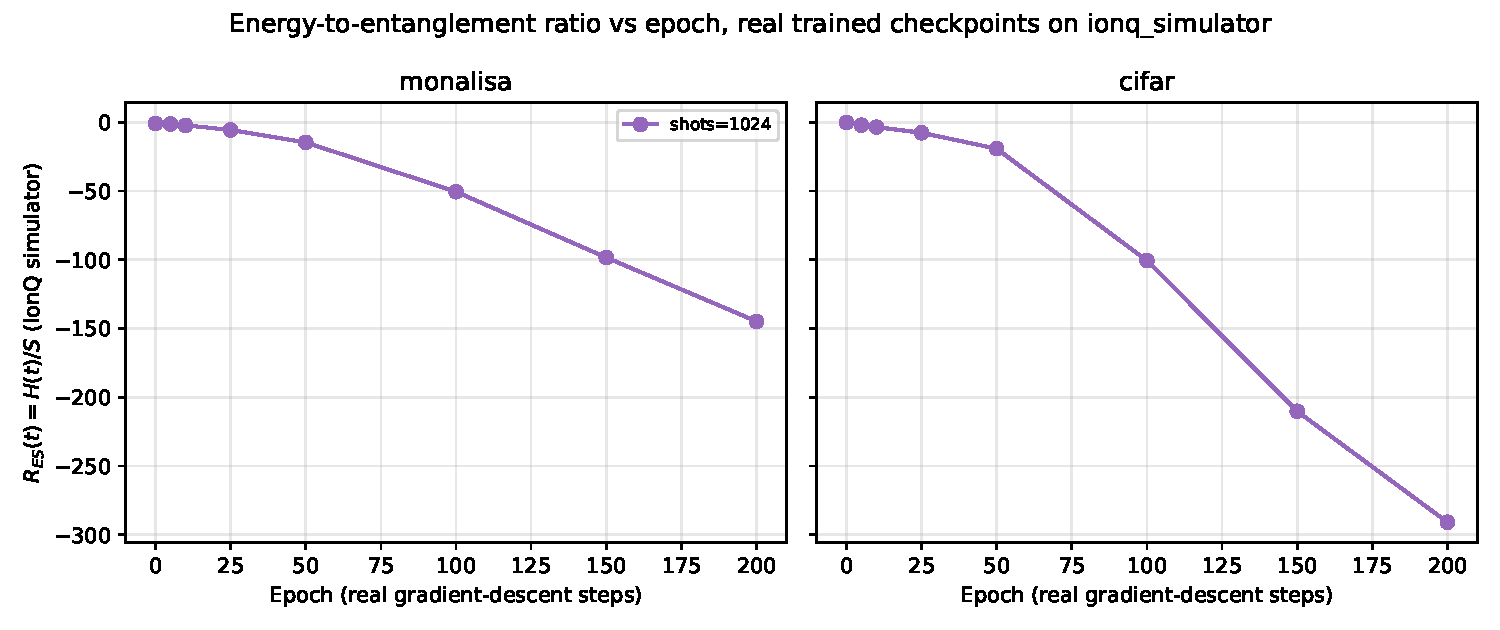
\includegraphics[width=\linewidth]{figures/checkpoint_ionq_energy_entanglement_ratio.pdf}
\caption{$R_{ES}(t)=H(t)/S$ from the same $N=6$ real trained checkpoints as Figure~\ref{fig:checkpoint_hardware_energy_entanglement}, Pauli bond correlators measured instead on the IonQ ideal cloud simulator (1024 shots, the only shot budget submitted for this diagnostic).}
\label{fig:checkpoint_ionq_energy_entanglement}
\end{figure}

Figure~\ref{fig:checkpoint_ionq_energy_entanglement} shows the resulting IonQ traces preserve the same monotonically decreasing shape as the IBM replay above and the noiseless-simulator traces of Figure~\ref{fig:critical_temperature}, for both images. As above, we do not apply the descriptive detection rule of Eq.~\ref{eq:critical_epoch} to these single-patch traces; this is an ideal cloud-simulator portability check, not an IonQ-QPU result.

\section{Discussion}

\subsection{Why the Physics-Informed Regularizer Was Inert}
\label{sec:regularizer_inert}
Table~\ref{tab:hamiltonian_controls} shows the Hamiltonian energy term is, if anything, a mild drag on reconstruction quality in the present system. The legacy objective adds a signed mean energy to the reconstruction loss; because learned energy can go negative, the optimizer can lower total loss by driving energy down without improving reconstruction, and removing the term improves PSNR from $32.24$ to $33.30$~dB. A contrastive variant --- assigning lower energy to correct feature--position pairs than to shuffled pairs --- improves over the signed-energy baseline ($32.84$~dB) but remains below its own no-energy-loss counterpart ($33.33$~dB), and ZZ-only observables ($32.88$~dB) show nearest-neighbor correlations are largely sufficient on their own. We read this as a case where the reconstruction loss already dominates the optimization signal at this model scale and dataset size: a physically motivated regularizer has room to help when it resolves an otherwise underdetermined objective, and here the pixel-fidelity loss alone is sufficiently informative that the extra term mostly adds noise to the gradient. This does not mean Hamiltonian regularization is never useful --- only that its value is conditional on the reconstruction loss being under-constrained, a condition this patch-level pixel task does not meet.

\begin{table*}[t]
\centering
\caption{Hamiltonian and observable-sector controls (single-seed). The energy objective is diagnostically useful but does not improve reconstruction accuracy.}
\label{tab:hamiltonian_controls}
\scriptsize
\begin{tabular}{p{0.30\textwidth}cccp{0.32\textwidth}}
\toprule
Experiment & MSE & PSNR (dB) & SSIM & Interpretation \\
\midrule
Legacy baseline, signed energy & $5.9771\times10^{-4}$ & 32.24 & 0.9919 & Standard energy-regularized run \\
No energy loss & $4.6772\times10^{-4}$ & 33.30 & 0.9937 & Removing energy improves PSNR \\
No observable noise & $5.3518\times10^{-4}$ & 32.72 & 0.9928 & Noise is not essential \\
Contrastive Hamiltonian core & $5.1975\times10^{-4}$ & 32.84 & 0.9930 & Stronger objective helps modestly vs. baseline \\
Contrastive, no energy loss & $4.6498\times10^{-4}$ & 33.33 & 0.9937 & Energy removal still performs best \\
ZZ-only observables & $5.1503\times10^{-4}$ & 32.88 & 0.9930 & Nearest-neighbor $ZZ$ correlations largely suffice \\
\bottomrule
\end{tabular}
\end{table*}

The order-parameter and energy-to-entanglement-ratio diagnostics of Sections~\ref{sec:phase_transition}--\ref{sec:critical_temperature} provide descriptive windows into training dynamics. Their detected epochs come from changes in measured model summaries, but the data-dependent threshold is not a calibrated statistical test and the results should not be interpreted as thermodynamic transitions.

\subsection{Task-Dependent Representational Scope}
\label{sec:dequant}
Whether a quantum feature map or kernel offers any advantage over a classical model is a property of the specific data and target, not a fixed property of the model class, and dequantization results have repeatedly shown that apparent quantum advantages on structured, low-entanglement classical data can be matched by classical algorithms once the right classical feature is identified \cite{Huang2021PowerData}. The restricted diagnostic of Section~\ref{sec:entanglement_necessity} is constructed so that the relevant structure is a genuine distant-element product raw or local features cannot represent under a fixed linear readout, and that is precisely the regime in which HVK's entangling channel separates. Natural image patches, at the resolution and patch size used in ordinary reconstruction, are a different regime --- low-entanglement, locally structured data where a linear or shallow classical readout is already close to sufficient. The companion supplementary study's held-out comparisons (Section~\ref{sec:ablation_relationship}) characterize exactly this second regime; together, the results delineate where the tested entangling representation does and does not yield a measurable benefit.

\subsection{Relationship to the Component-Wise Ablation Study}
\label{sec:ablation_relationship}
The results above establish what HVK is and several of its provable or verified properties. A separate, equally important question --- whether its feature map improves reconstruction on real, \emph{held-out} images under a resource-matched multi-seed protocol --- is answered in the companion document, \textit{Supplementary Material for the Hamiltonian Vision Kernel: Resource-Matched Ablations, Validation, and Reproducibility}. On held-out CIFAR-10, local-observable and raw-linear controls reach $18.80\pm1.42$~dB against HVK2D's $18.12\pm1.54$~dB; after aggregating held-out images within each split, the HVK2D-minus-control difference is $-0.68$~dB (bootstrap 95\% CI $[-0.91,-0.46]$~dB; Wilcoxon $p=0.0625$, $n=5$ seeds), with the same numerical direction on five further real datasets. Thus the tested HVK map is informative but is not shown to outperform the simpler maps on ordinary held-out reconstruction. We report this as a rigorous complement: it delineates the tested boundary of the positive entanglement and symmetry results and records the provenance checks that prevented exploratory artifacts from becoming claims.

\subsection{Topology Alignment as an Inductive Bias}
\label{sec:topology}
Aligning the latent interaction graph with image-patch adjacency (HVK2D vs.\ HVK1D) is a plausible architectural inductive bias: on \textit{Monalisa}, 2D HVK exceeds its 1D counterpart by $5.98$~dB ($40.70$ vs.\ $34.72$~dB). The companion supplementary study tests this hypothesis more directly under matched held-out conditions. Its real-circuit subset (3 seeds, 3 held-out CIFAR-10 images) gives an HVK1D-minus-HVK2D mean PSNR difference of $0.16$~dB; after averaging images within seed, the bootstrap 95\% CI is $[-0.38,0.46]$~dB and the seed-level Wilcoxon test gives $p=0.50$. HVK2D completes the matched 90-step runs in roughly half the wall-clock time. A broader five-seed surrogate comparison across CIFAR-10, Fashion-MNIST, and PathMNIST likewise finds numerically small topology differences (at most $0.07$~dB in mean PSNR). At the tested scale, topology therefore appears to be primarily a resource-cost choice rather than a reliable accuracy advantage; these tests do not establish formal equivalence.

\subsection{Architectural Differentiation Matrix}
Table~\ref{tab:differentiation} contrasts HVK's structural properties against reference frameworks. Its distinguishing features --- a Pauli-correlator latent space, 2D Fourier positional bias with enforced $D_4$ pooling, and a Hamiltonian energy diagnostic --- are documented and scoped in the preceding sections.

\begin{table*}[t]
\centering
\caption{Architectural differentiation from representative baseline designs.}
\label{tab:differentiation}
\begin{tabular}{lcccc}
\toprule
Axis & Conv. AE baseline & GAN baseline & Register-based QAE & HVK (ours) \\
\midrule
Latent representation & Continuous $\mathbb{R}^d$ & Continuous $\mathbb{R}^d$ & Quantum register & Pauli-correlator vector \\
Spatial bias & Convolutional & Convolutional & Encoding-dependent & 2D Fourier encoding \\
Auxiliary objective & Bottleneck/reconstruction & Adversarial loss & Fidelity/reconstruction & Hamiltonian diagnostic \\
Enforced group symmetry & Not in baseline & Not in baseline & Not in reference design & $D_4$ observable pooling \\
Evaluated role & Reconstruction & Reconstruction & Compression & Reconstruction + diagnostics \\
\bottomrule
\end{tabular}
\end{table*}

\subsection{Validated Scope and Next Steps}
\label{sec:limitations}
\begin{itemize}
    \item Every reconstruction result in this paper (Sections~\ref{sec:sameset_results}--\ref{sec:no_generalization}) is per-image trained, not held-out generalization; the companion supplementary study's held-out protocol is the appropriate evidence for a generalization claim, and its finding that local/raw maps match or exceed the tested HVK map under the shared readout should be read alongside the architecture-level results here.
    \item The $D_4$-pooled map (Section~\ref{sec:d4}) is currently a feature-grid-level construction and numerical diagnostic, not yet integrated into the trainable end-to-end reconstruction pipeline; doing so is concrete future work (Section~\ref{sec:conclusion}).
    \item The entanglement-necessity result (Section~\ref{sec:entanglement_necessity}) is scoped to a task deliberately constructed to require nonlocal structure; it does not by itself establish an advantage on ordinary natural-image reconstruction (see Section~\ref{sec:dequant}).
    \item The hardware pilot (Section~\ref{sec:hardware_pilot}) is a five-image, single-trial, unmitigated pilot, not a statistically resolved hardware benchmark.
    \item The original exploratory training-dynamics traces were withdrawn after a provenance audit (Section~\ref{sec:phase_transition}); the corrected, noise-free multi-seed replacement is a small-sample diagnostic (2 images $\times$ 2 seeds/dataset, 24 runs across six datasets) with mixed, not universal, detection ($16/24$), and should be read at that scope.
    \item The matched real-circuit topology comparison uses only 3 seeds and 3 held-out images per topology; the broader five-seed comparison is surrogate-based. These results support a resource-cost interpretation but do not establish formal equivalence of the topologies.
\end{itemize}

\section{Conclusion}
\label{sec:conclusion}
We presented the Hamiltonian Vision Kernel, a physics-informed hybrid quantum--classical image autoencoder distinguished by a Pauli-correlator latent space, an enforced and numerically verified $D_4$-equivariant observable-pooling extension, and a learnable graph-Hamiltonian energy diagnostic. Independently of reconstruction quality, we established two structural results at the tested scope: a provable $D_4$ symmetry construction (equivariance error $9.57\times10^{-17}$) and a restricted entanglement-sensitive result on a task requiring nonlocal structure, where pair observables are necessary within the tested fixed-readout feature class ($R^2=0.9735$ vs.\ $R^2\leq0.02$ for non-entangling controls). We further reported a real IBM Quantum hardware reconstruction pilot: replaying trained checkpoints without retraining yielded $25.90$--$31.52$~dB PSNR from hardware measurements. This pilot establishes feasibility at its five-image, single-trial scope rather than a general hardware-performance claim.

A companion supplementary study reports a separate, rigorous question: does the tested HVK feature map improve reconstruction on held-out real images under resource-matched controls? It does not at the evaluated scale; local/raw maps match or exceed it under the same fitted readout. This is not in tension with the structural results here. Instead, it separates them from an ordinary-reconstruction advantage: entangling observables separate only on the tested nonlocal target, and group pooling guarantees equivariance without establishing an accuracy gain. We consider this carefully measured boundary to be a constructive contribution alongside the architecture itself.

Future work should integrate the $D_4$-pooled map into an end-to-end trainable pipeline (currently a feature-grid-level construction, Section~\ref{sec:limitations}); scale the hardware pilot toward a statistically resolved benchmark with error mitigation and repeated trials; search for further real-world tasks with genuine nonlocal structure where HVK's restricted entanglement-sensitive separation translates into a reconstruction advantage; and extend the resource-matched, leakage-audited evaluation protocol used in the companion supplementary study to other hybrid quantum vision architectures.

\section*{Data and Code Availability}
The source code, experiment drivers, machine-readable result summaries, validation arrays, and figure inputs supporting this study are included in the accompanying repository. The file \path{project_artifacts/submission_claim_audit.json} maps the three numerical headline claims to their retained source artifacts, and automated tests verify those mappings. Dataset provenance and access routes are cited in the manuscript and detailed in the supplementary artifact map. IBM Quantum job identifiers and reconstructed outputs are retained; as disclosed in the supplement, the raw account-usage service response was not serialized, so the reported quota change is an execution-log record rather than a repository-recomputable measurement.

\section*{Acknowledgements}
We thank the maintainers of the open-source scientific computing libraries used in this work.

\begin{thebibliography}{99}
\bibitem{Cerezo2021} M. Cerezo et al., ``Variational quantum algorithms,'' \textit{Nature Reviews Physics}, vol. 3, no. 9, pp. 625--644, 2021.
\bibitem{Tilly2022} J. Tilly et al., ``The Variational Quantum Eigensolver: A review of methods and best practices,'' \textit{Physics Reports}, vol. 986, pp. 1--128, 2022.
\bibitem{Bauer2020} B. Bauer, S. Bravyi, M. Motta, and G. K.-L. Chan, ``Quantum Algorithms for Quantum Chemistry and Quantum Materials Science,'' \textit{Chemical Reviews}, vol. 120, no. 22, pp. 12685--12717, 2020.
\bibitem{Chakraborty2018} S. Chakraborty, S. B. Mandal, and S. H. Shaikh, ``Quantum image processing: challenges and future research issues,'' \textit{International Journal of Information Technology}, vol. 14, no. 1, pp. 475--489, 2022, doi: 10.1007/s41870-018-0227-8.
\bibitem{Zhou2017} R. Zhou, W. Hu, P. Fan, and H. Ian, ``Quantum realization of the bilinear interpolation method for NEQR,'' \textit{Scientific Reports}, vol. 7, no. 1, p. 2511, 2017.
\bibitem{Yao2017} X. Yao et al., ``Quantum Image Processing and Its Application to Edge Detection: Theory and Experiment,'' \textit{Physical Review X}, vol. 7, no. 3, p. 031041, 2017.
\bibitem{Cirac2021} J. I. Cirac, D. Pérez-García, N. Schuch, and F. Verstraete, ``Matrix product states and projected entangled pair states: Concepts, symmetries, theorems,'' \textit{Reviews of Modern Physics}, vol. 93, no. 4, p. 045003, 2021.
\bibitem{Latorre2005} J. I. Latorre, ``Image compression and entanglement,'' arXiv:quant-ph/0510031, 2005.
\bibitem{Han2018} Z. Han, J. Wang, H. Fan, L. Wang, and P. Zhang, ``Unsupervised Generative Modeling Using Matrix Product States,'' \textit{Physical Review X}, vol. 8, no. 3, p. 031012, 2018.
\bibitem{Fei2021} S. M. Fei, ``Compressed Sensing Based on Tensor Network Machine Learning,'' \textit{Physical Science \& Biophysics Journal}, vol. 5, no. 1, Art. no. 000174, 2021, doi: 10.23880/psbj-16000174.
\bibitem{Guala2023} D. Guala et al., ``Practical overview of image classification with tensor-network quantum circuits,'' \textit{Scientific Reports}, vol. 13, no. 1, p. 4427, 2023.
\bibitem{Haga2024} A. Haga, ``Quantum annealing-based computed tomography using variational approach for a real-number image reconstruction,'' \textit{Physics in Medicine and Biology}, vol. 69, no. 4, Art. no. 04NT02, 2024, doi: 10.1088/1361-6560/ad2155.
\bibitem{Zhai2025} X. Zhai, T. Xiao, J. Huang, J. Fan, and G. Zeng, ``Quantum neural compressive sensing for ghost imaging,'' \textit{Physical Review Applied}, vol. 23, no. 1, p. 014018, 2025.
\bibitem{Nau2023} M. A. Nau, A. H. Vija, W. Gohn, M. P. Reymann, and A. Maier, ``Exploring the Limitations of Hybrid Adiabatic Quantum Computing for Emission Tomography Reconstruction,'' \textit{Journal of Imaging}, vol. 9, no. 10, p. 221, 2023.
\bibitem{Xu2021} R. Xu, X. Wang, K. Chen, B. Zhou, and C. C. Loy, ``Positional Encoding as Spatial Inductive Bias in GANs,'' in \textit{Proceedings of the IEEE/CVF Conference on Computer Vision and Pattern Recognition (CVPR)}, 2021, pp. 13564--13573.
\bibitem{Araz2022} J. Y. Araz and M. Spannowsky, ``Classical versus quantum: Comparing tensor-network-based quantum circuits on Large Hadron Collider data,'' \textit{Physical Review A}, vol. 106, no. 6, p. 062423, 2022.
\bibitem{Slabbert2024} D. Slabbert and F. Petruccione, ``Hybrid Quantum-Classical Feature Extraction approach for Image Classification using Autoencoders and Quantum SVMs,'' arXiv:2410.18814, 2024.
\bibitem{Liu2022} Z. Liu, P.-X. Shen, W. Li, L.-M. Duan, and D.-L. Deng, ``Quantum capsule networks,'' \textit{Quantum Science and Technology}, vol. 8, no. 1, p. 015016, 2022.
\bibitem{Shi2022} J. Shi, W. Wang, X. Lou, S. Zhang, and X. Li, ``Parameterized Hamiltonian Learning With Quantum Circuit,'' \textit{IEEE Transactions on Pattern Analysis and Machine Intelligence}, vol. 45, no. 5, pp. 6086--6095, 2022.
\bibitem{Preskill2018} J. Preskill, ``Quantum Computing in the NISQ era and beyond,'' \textit{Quantum}, vol. 2, p. 79, 2018.
\bibitem{Havlicek2019} V. Havl{\'i}{\v c}ek, A. D. C{\'o}rcoles, K. Temme, A. W. Harrow, A. Kandala, J. M. Chow, and J. M. Gambetta, ``Supervised learning with quantum-enhanced feature spaces,'' \textit{Nature}, vol. 567, no. 7747, pp. 209--212, 2019.
\bibitem{Stoudenmire2016} E. M. Stoudenmire and D. J. Schwab, ``Supervised Learning with Tensor Networks,'' in \textit{Advances in Neural Information Processing Systems}, vol. 29, 2016.
\bibitem{Cohen2016} T. Cohen and M. Welling, ``Group Equivariant Convolutional Networks,'' in \textit{Proceedings of the 33rd International Conference on Machine Learning}, PMLR, vol. 48, 2016, pp. 2990--2999.
\bibitem{Meyer2023} J. J. Meyer, M. Mularski, E. Gil-Fuster, A. A. Mele, F. Arzani, A. Wilms, and J. Eisert, ``Exploiting Symmetry in Variational Quantum Machine Learning,'' \textit{PRX Quantum}, vol. 4, p. 010328, 2023.
\bibitem{Huang2020Shadows} H.-Y. Huang, R. Kueng, and J. Preskill, ``Predicting many properties of a quantum system from very few measurements,'' \textit{Nature Physics}, vol. 16, pp. 1050--1057, 2020.
\bibitem{IonQBackends} IonQ, ``Backends,'' \textit{IonQ Quantum Cloud Documentation}. [Online]. Available: \url{https://docs.ionq.com/user-manual/backends}. Accessed: Jul. 24, 2026.
\bibitem{Huang2021PowerData} H.-Y. Huang, M. Broughton, M. Mohseni, R. Babbush, S. Boixo, H. Neven, and J. R. McClean, ``Power of data in quantum machine learning,'' \textit{Nature Communications}, vol. 12, no. 1, p. 2631, 2021.
\bibitem{Krizhevsky2009} A. Krizhevsky, ``Learning multiple layers of features from tiny images,'' University of Toronto, Technical Report, 2009.
\bibitem{LeCun1998} Y. LeCun, L. Bottou, Y. Bengio, and P. Haffner, ``Gradient-based learning applied to document recognition,'' \textit{Proceedings of the IEEE}, vol. 86, no. 11, pp. 2278--2324, 1998, doi: 10.1109/5.726791.
\bibitem{Xiao2017} H. Xiao, K. Rasul, and R. Vollgraf, ``Fashion-MNIST: A novel image dataset for benchmarking machine learning algorithms,'' arXiv:1708.07747, 2017.
\bibitem{Yang2023} J. Yang et al., ``MedMNIST v2---A large-scale lightweight benchmark for 2D and 3D biomedical image classification,'' \textit{Scientific Data}, vol. 10, Art. no. 41, 2023, doi: 10.1038/s41597-022-01721-8.
\end{thebibliography}

\end{document}
